% Chapter 5

\chapter{Implementation and Evaluation} % Main chapter title
\label{Evaluation} % For referencing the chapter elsewhere, use \ref{Chapter1} 

\section{SLA Frontend}

\subsection{KPIs and Infrastructure Data}
As introduced in chapter \ref{Cloud KPIs}, KPIs are widely used to measure and overview computing environments. In this implementation and evaluation environment data has been collected via the Ganglia \cite{Ganglia} distributed monitoring system, which is based on a hierarchical design and targeted at federations of clusters. Figure \ref{fig:monidata} below shows the Ganglia interface with collected infrastructure data from our OpenStack Cloud environment.

\begin{figure}[ht]
	\centering
	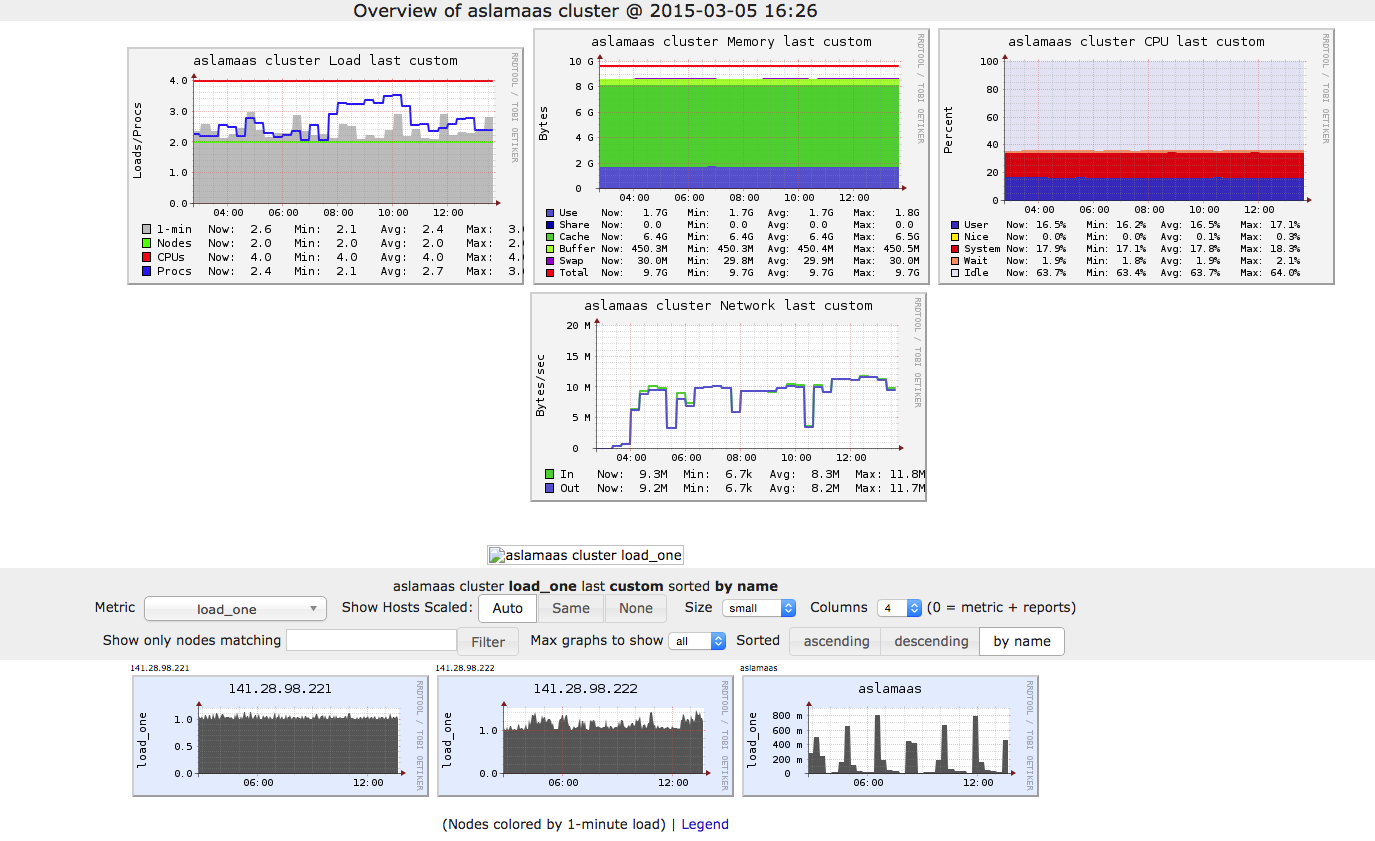
\includegraphics[width=0.7\linewidth]{chapters/chapter5/fig/monidata_cluster}
	\caption{Ganglia Cluster Overview}
	\label{fig:monidata}
\end{figure}

Here it can be seen how core KPIs, such as memory usage, cpu load, process load and network traffic is monitored. The test environment consisted of two worker nodes. Here different types of load scenarios where used by running an request generator, which accessed the services. This data was then collected and archived during a 6 months period.

\begin{figure}[ht]
	\centering
	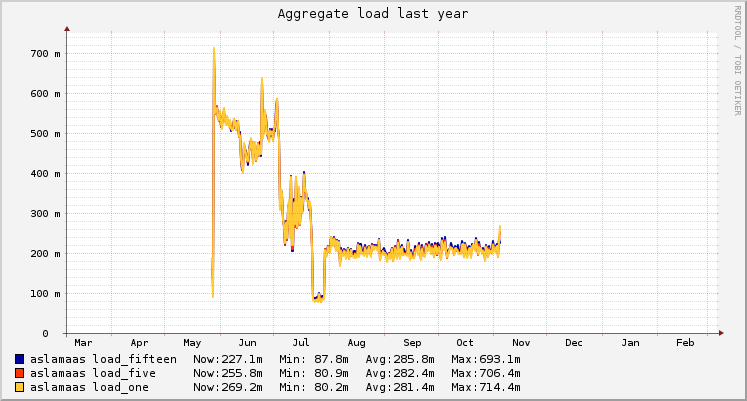
\includegraphics[width=0.7\linewidth]{chapters/chapter5/fig/monidataloadlast}
	\caption{Cluster Load Aggregation}
	\label{fig:monidata2}
\end{figure}

Figure \ref{fig:monidata2} above shows the aggregated load graph for the cluster during the testing period. All data was as well collected in a time series data store. Additional in the scenarios described in later sections, simulated workloads have been used to generate a repeatable and comparable environment. Various typical workload scenarios were depicted, such as a burst load scenario, which could also be observed on the live system due to real life usage.


\subsection{GUI}
In order to interact with the implementation a GUI was designed to facilitate the use and the feel of the prototypical system.

\begin{figure}[ht]
	\centering
	\includegraphics[width=0.7\linewidth]{chapters/chapter5/fig/GUI}
	\caption{First GUI Mockup}
	\label{fig:gui}
\end{figure}


\begin{figure}[ht]
	\centering
	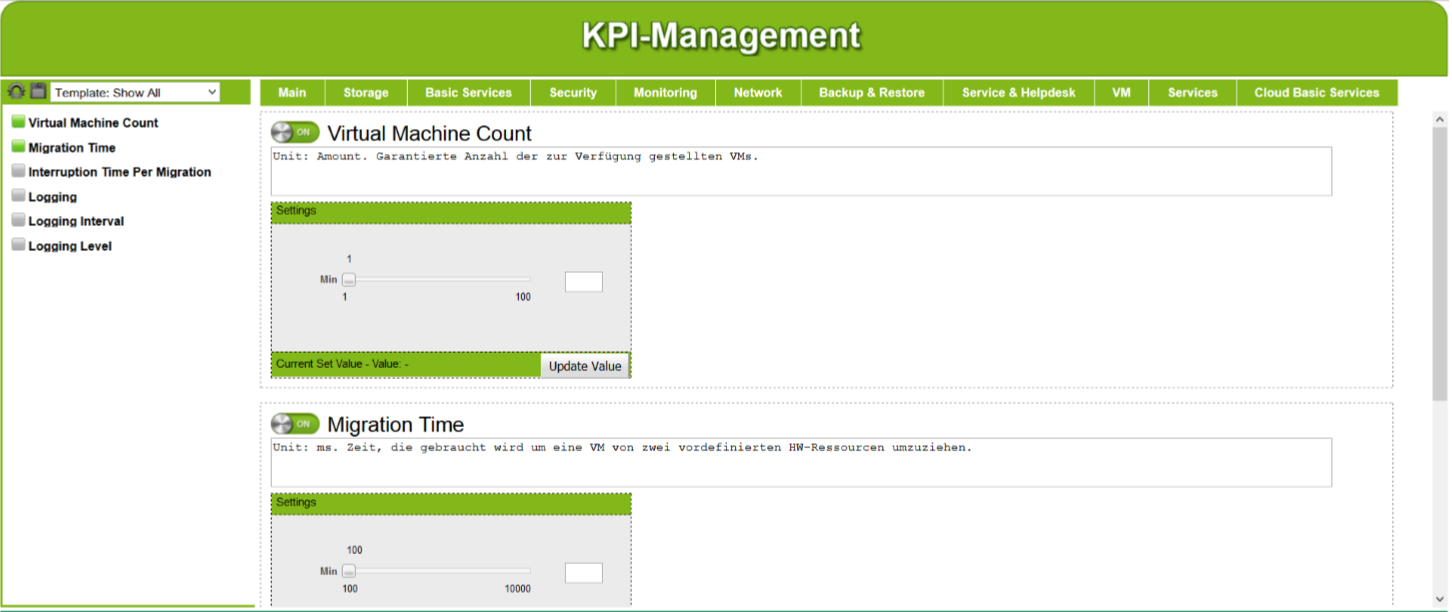
\includegraphics[width=0.7\linewidth]{chapters/chapter5/fig/Gui1}
	\caption{Final GUI}
	\label{fig:gui1}
\end{figure}


\begin{figure}[ht]
	\centering
	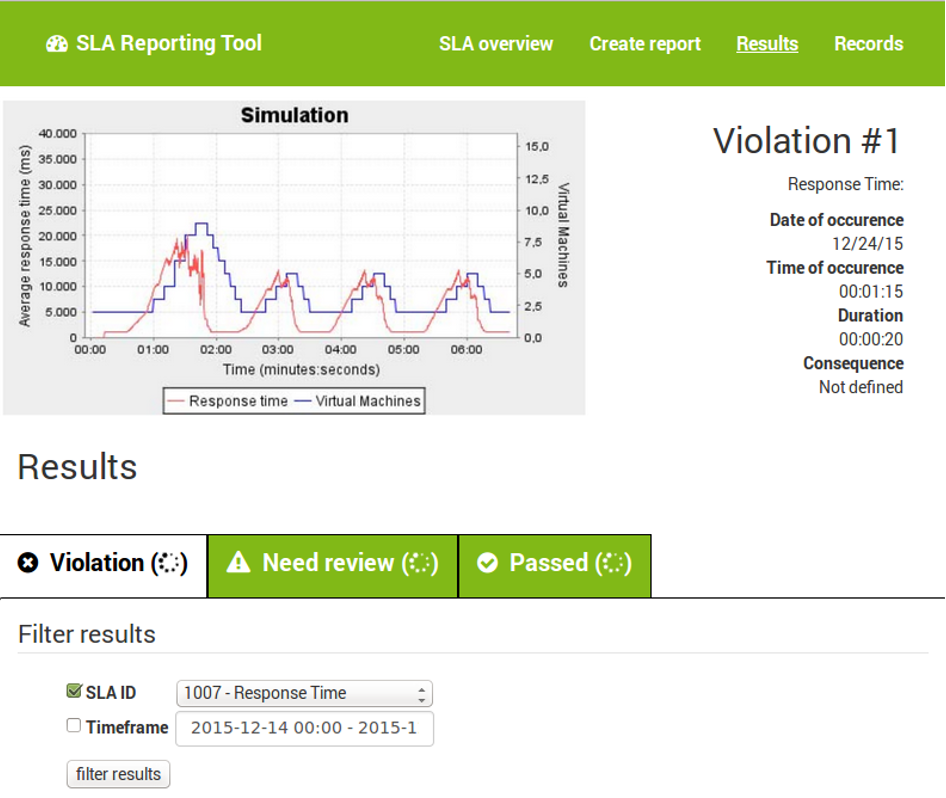
\includegraphics[width=0.7\linewidth]{chapters/chapter5/fig/Gui2}
	\caption{SLA Violation Report}
	\label{fig:gui2}
\end{figure}


\subsection{A-SLO-A}
The reference implementation of the SLO-A format is based on the abstract SLA* model, developed within the SLA@SOI project cite{Kearney2011b}. The SLA* model is an abstraction layer and follows the description of the Meta Object Facility (MOF), specified by the Object Management Group (OMG). MOF describes a special meta data architecture and itself uses the highest abstraction layer M3. The SLA* model is on layer M2, this correspondences to the Platform Specific Model (PIM). The SLO-A Format is one abstraction layer below (M2). This describes the Platform Specific Model (PSM). So the SLO-A Format is on the same level like SLA(T) description of the SLA@SOI project, as shown in Figure \ref{fig:mbd_SLOA}.
\begin{figure}[ht]
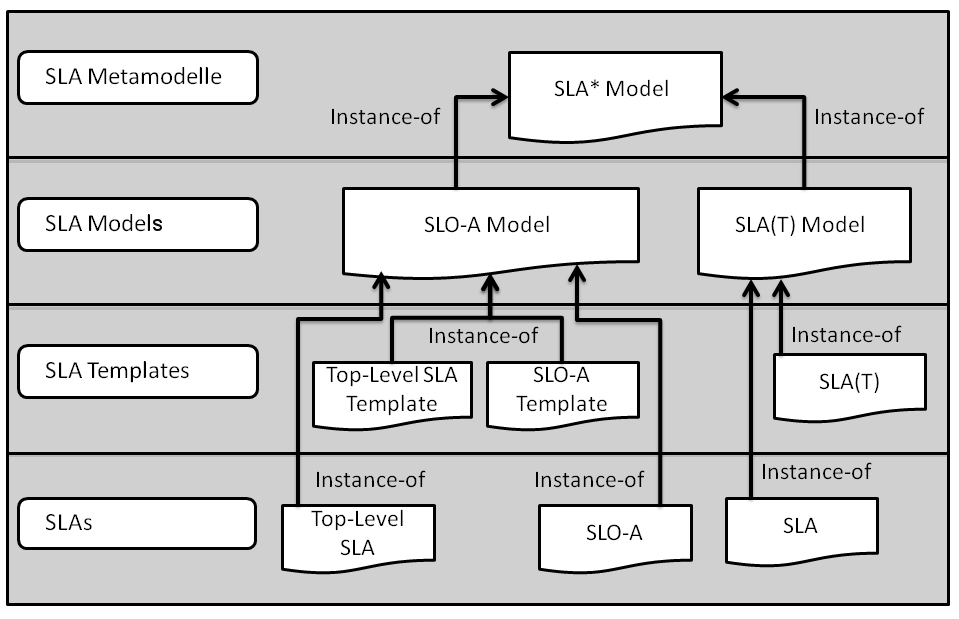
\includegraphics[width=0.5\textwidth]{fig/Modellbasierte_Entwicklung_Instanz.png}
\caption{Model Based Development of SLO-A}
\label{fig:mbd_SLOA}
\end{figure}
For the reference model of SLO-A it has not be used the primitive data types of the SLA* model instead the EMF data types of the Eclipse module Ecore are used. This was necessary to get a functional prototype.

The main goal of the format is to develop an adaptable, adequate machine readable agreement which is legally binding. To get customer-oriented, runtime-adaptable SLAs it is first divided into a static and a dynamic part. The static part, like contract partner IDs, addresses, etc. is important, but more interesting is the part changeable during runtime, focused on SLOs like max. scaling limit, backup period, etc. This dynamic SLA part must be monitor-able and controlled by the customer.

Within the SLO-A format it is possible to define Top-Level SLAs and SLO-Agreements (SLO-As) which are single and dedicated for each SLO.

\subsubsection{Top-Level-SLA to a SLO}
\begin{figure}[ht]
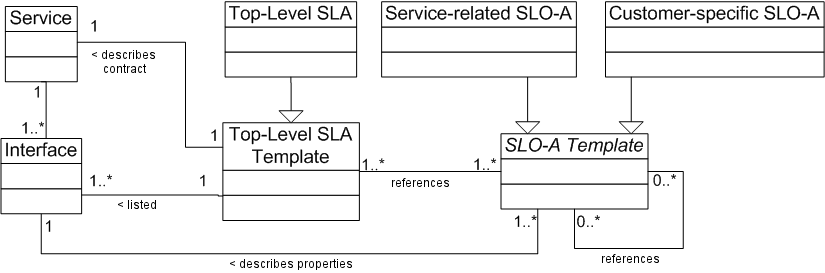
\includegraphics[width=0.5\textwidth]{fig/sloa_arch_allg.png}
\caption{Overview of SLO-A Format}
\label{fig:overview_sloa}
\end{figure}
All Top-Level SLAs and SLO-Agreements are based on a appropriated template (see Fig. \ref{fig:overview_sloa}. Also a Top-Level SLA always is displayed by a service which can have one or more interfaces, which are the base of the agreement. On the contrary a SLO-A is not based directly on a service only with the interfaces. Here technically or contractually responsibilities effect can be modelled.

Resulting characteristics of the model:
\begin{itemize}
\item Technical services are characterized by a one to one assignment from a Top-Level-SLA to an SLO template, it's a so called service oriented SLO template. Also SLO-A templates can be referenced to another SLO-A template and build a hierarchy.
\item SLO-As can be grouped by a higher SLO-A or a Top-Level SLA. This builds a hierarchical tree where each entity is referenced to the next higher SOL-A with an UUID and a naming convention. So a an entity directly references the low SLO-A and monitoring can be done over all. 
\end{itemize}
\begin{figure}[ht]
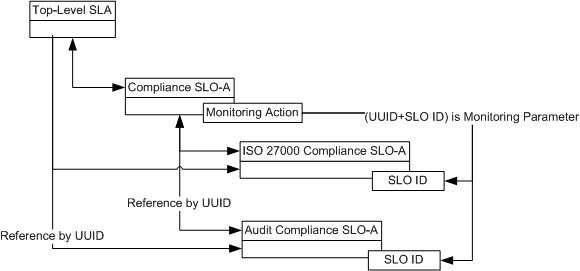
\includegraphics[width=0.5\textwidth]{fig/sloa_arch_refs.png}
\caption{Example of References within SLO-A}
\label{fig:example_sloa}
\end{figure}

\subsubsection{Top-Level SLAs and Top-Level SLA Templates}
Basically the Top-Level SLA comprehend static contractual informations and only few dynamic informations. Also there can be made references to outsourced documents like general terms and conditions. A Top-Level SLA necessary must have informations about accounting of services, IT continuity plan, service development plan, terminology, escalation plans, guidelines for priorities, responsibilities of both customer and company, data of both parties, service times, accomplishment penalties, signing, an ID, how reports have to been done and how the were displayed in which frequenz, the interfaces with ID and description, references of SLO-as with UUID and naming convention, and the termination reason.

For a legally binding SLO-A have to to contain a SLO-A identifier, contact data, service time. Also the SLO itself with an ID, a value and data type which has exactly one interface, which priority, if needed the allocation to other SLO with their interfaces, the boundary an marginal values. The SLO-A additionally should contain the SLO-A reference, the accounting, accomplishment penalties, monitoring, how and with with interface it is done, how the reporting is done and the termination clause.

\subsubsection{Workflow for a Top-Level Sla or SLO-A}
To generate a Top-Level SLA or a SLO-A , the customer first has to fill in the customer data,  servie times, how it will be payed and how it should be reported with which interfaces. In comparison to a SLO-A there also has to be filled in how it should be monitored. After that a decision is made if its an standard template or a customer oriented template. In order its standard all information will be checked and if necessary it is asked for correction. Otherwise if its an customer oriented template, it is asked for a special template.  If the value verification is accepted at the Top-Level SLA, all SLO-A are filled in and the inferior references are build. At the SLO-A template the reference is to the higher entity is build directly. After that the templates got signed and the contract are ready. 

The incident an change management are mapped as a inferior grouped SLO-A, so they can be used as KPI. An extension of conditions and modality can involve more actions, which always have a condition, guidelines and postcondition. They describe how the action will be triggered.

\subsubsection{Reference Implementation}\label{section_ref_impl}
The SLA Format implementation is done as part of master thesis by Ralf Teckelmann at the HS Furtwangen University \cite{Teckelmann2012}. There have been made many extensions to the SLA Templates proposed by the SLA@SOI project.
One important part of a SLA Template (see Figure \ref{fig:overview_SLAT}) is the extension of the attribute {\it Type}. It differs from the Type of the SLA Template by the possibility to have 3 values: {\it top-level}, {\it service} and {\it customer}. This causes an 'IF' clause to load a concrete structure into the SLA template or SLA. So that means, when {\it Type} is either {\it service} or {\it customer} it is a SLO-A Template or SLO-A. For the unique identification the {\it UUID} attribute is used. Also the model version can be found in the attribute {\it modelVersion}.
The next subsections discuss the main features of the SLO-A Model in detail.

\subsubsection{SLAs and SLA Templates}
As described in last chapter the documentation is as following: There are two segments, that contains the documentation part of the SLA/SLO-A Templates. The first segment {\it descriptions} keeps the general terms of the agreement. The second segment {\it fuDocs} (shortcut for further Documents) contains the interface description. Both structures will be described later. Normally it is possible to use SLA and SLA Templates without agreement term segment, but for compatibility reasons to SLA* respectively SLA(T) this segment is included.
\begin{figure}[ht]
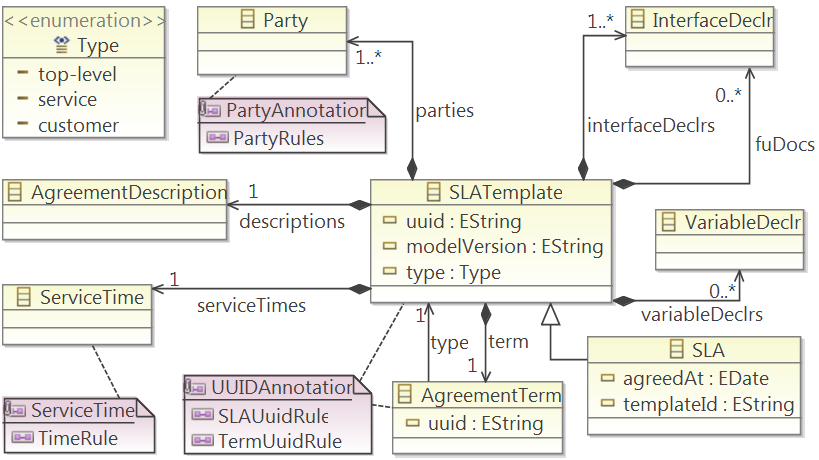
\includegraphics[width=0.5\textwidth]{fig/sloa_slas_sla-templates.png}
\caption{Overview of SLA Template, a modified and extended SLA(T) model \cite{Lambea2011}}
\label{fig:overview_SLAT}
\end{figure}

\subsubsection{Description of Agreements}
The class {\it Agreement Description} as segment {\it description} of SLA templates and SLA has also its own structure. This is a different to the SLA* model. In SLA(T) there exists only a {\it ServiceDescription} segment without further information. In SLO-A Format the segment {\it descriptions} contains exactly one element of the class {\it Property} with its segment {\it entries}. These {\it entries} use the class {\it Entry} with its two attributes {\it key} and {\it value}. The attribute {\it key} contains the type of the following document in the attribute {\it value}. The type can be either a {\it CoverageDescr}, a {\it AgrementDescr} or a {\it Disclaimer}. The information itself is in the attribute {\it value}.

\subsubsection{Time Frames}
The next segment of the class {\it SLATemplate} is the {\it serviceTimes}. It describes the time the service must be available. The segment uses the class {\it ServiceTime} one time. All times are save there. This is also a different to the implementation in the SLA* model. In the SLA* model only a start and a stop time defined. This is not enough. So the SLA-O Format creates the class {\it ServiceTime} which holds in its segment {\it serviceTimePairs} a list of different time intervals, where an interval contains a pair of a class {\it entry}, where the time definition is stored.

\subsubsection{Parties}
The contracting parties will be placed in the segment {\it parties} of the class {\it SLATemplate}. Here are used the original class {\it party} of the SLA* model. It contains a contact point with all required information. Also the class {\it STND} is included which holds information about the {\it agreementRole}. This is normally either the {\it provider} or the {\it consumer}. Also it is possible to store {\it Operatives}. These are contact persons, which can be directly assosiated to {\it Actions}. The annotation {\it PartyRules} describes conditions when information be available in a SLA or SLA template, this is a deviation to the SLA* model.

\subsubsection{Signatures in SLAs and SLA Templates}
A complete new attribute is in the class {\it SLATemplate} the segment {\it ProviderSignature} and in the class  {\it SLATemplate} the segment {\it customerSignature}. This contains the signature of the corresponding party. This feature allows it, to sign a SLA online. Is a SLA accepted by the customer and/or the provider, the corresponding signature will be added to the {\it SLA} (segment {\it customerSig}) and {\it SLATemplate} (segment {\it providerSig}).

\subsubsection{Interface Declaration}
The interface declaration is part of the service description and is used to connect the interfaces of a service and the SLOs. Also for the reference of further documents it is needed. There exists two ways to implement that, but both uses the abstract class {\it interface}. First is done by the resource oriented
interface {\it ResVersion}. This is used to keep further external documentation in the segment {\it endpoints}. The class {\it Endpoints} contains the three attributes {\it location}, {\it id} and {\it protocol}, to describe how to access the document. The {\it location} represents the location of the file, for example an URL, the {\it protocol} gives the required protocol to access the file, for an URL it could be {\it HTTP} or {\it HTTPS}. The {\it id} contains an unique identifier for the document. The attribute {\it refProvider} describes, who deposit the document. Also the segment {\it interface} repesented by the class with the same name contains through the class {\it ResourceType} the type of the document. This is in upper letter the type of the document. This is for PDF document the shurtcut 'PDF'.
The other possibility to describe an interface is the class {\it SpecVersion}. Here a Web Service can be defined by WSDL (Web Service Description Language). This is also part of the SAL* interface specification. Therefore the classes {\it InterfaceDeclr}, {\it InterfaceSpecification}, {\it InterfaceOperation} and {\it InterfaceProperties} are needed. The class {\it InterfaceSpecification} contains the {\it id} of the specification and in the segment {\it operations} are deposit all the operations of the WSDL part.
\begin{figure}[ht]
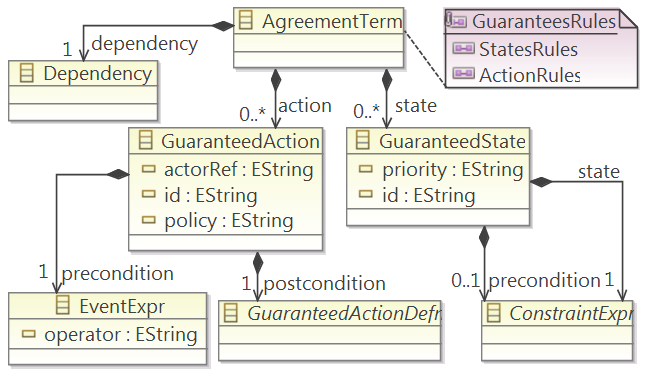
\includegraphics[width=0.5\textwidth]{fig/sloa_agreement_term.png}
\caption{Overview of Agreement Terms}
\label{fig:overview_AT}
\end{figure}

\subsubsection{Aggreement Terms}
The {\it AgreementTerm} segment is the core part of the SLA* Agreement and is a segment of {\it SLATemplate}, because it contains the states {\it GuaranteedStates} and the resulting actions {\it GuaranteedAction}. A state describes the relation between a SLO and a measure point based on a interface. In general states contains an attribute {\it priority}. Both (stats and actions) have conditions. The actions must have a {\it precondition} and a {\it postcondition}, a state can have many {\it preconditions}. The representation of conditions happens by the ground expressions of the SLA* model. The actions have an attribute {\it actorRef}. This field contains the unit, who is responsible to work on it. The class {\it AgreementTerm} is contained in the segment {\it term} of the top level SLAs or SLO-As. This is a difference between the SLA* model and the SLO-A Format. Important is, that the class {\it AgreementTerm} can have only a segment {\it GuaranteedStates}, when the {\it type} is not {\it top-level}. Therefore are exists three state rules:
\begin{itemize}
\item A Top-Level SLA (Template) does not hold any states
\item An SLO-A (Template) can hold one or more states
\item An SLO-A (Template) without a state is a grouping KPI
\end{itemize}
For {\it ActionRules} it is essential that a Top-Level SLA (Template) or a SLO-A (Template) can hold any number of actions.

\subsubsection{Dependencies}
The Dependencies of the documents itself is solved simple with the classes {\it Dependency} and {\it Property}. Also there are no existing solution in the SLA* model or SLA(T). The idea behind this is, to set the documents itself in relation. All Agreement Term can have many superordinate (segment {\it depending})  and subordinate (segment {\it anteceding}) Terms over the class {\it Dependency} as segment {\it dependency}. To store the information below the class {\it Dependency} the class {\it Property} is used. The attribute {\it key} contains the name and the attribute {\it value} references the document either as URI or as UUID.
Also rules can be applied. Important is the{\it CustomerSLO-ARule}. This allows for non customer SLO-A (see attribute {\it type}) only exactly one entry for {\it anteceding}. This structure is quiet simpler than the mechanism in the SLA* model. 

\subsubsection{Service Level Objectives}
The description of Service Level Objectives contains two components. The first component is the declaration of objectives, its value and the threshold. The threshold will be defined by the variable declaration. This is a mechanism to define a {\it name}, a {\it value} and a {\it data type}. Also the treshold values will be added, that all required information are available. The state definition creates a connection between the in the SLO defined value and at the runtime estimated value (measure point). The second component of the SLAs is the state definition. This is done by the class {\it GuaranteedState}. It has a {\it Priority}, this can be optional set. This class connects the values defined in the SLO and the measured real time values. These information are called measure point. Important is that the name of a defined interface and a UUID of a top level template are required. This relation is known by the SAL* model but was extended. An association to an interface of a SLO-A is possible by storing an UUID of the top level SLA.
\begin{figure*}[ht]
\begin{center}
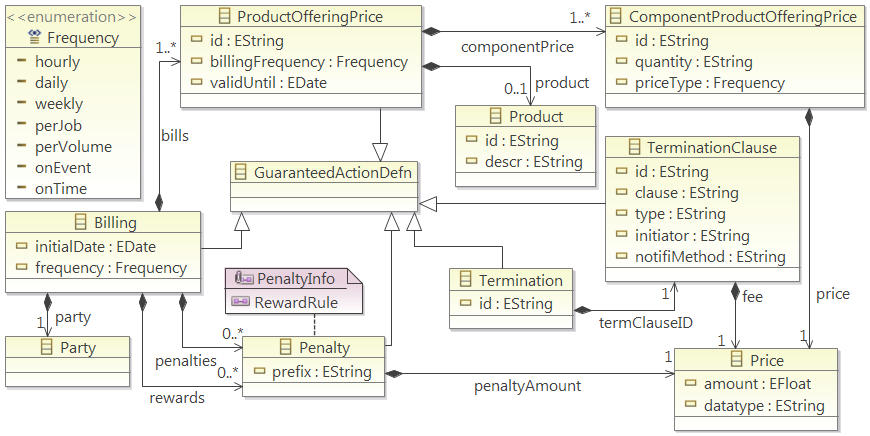
\includegraphics[width=0.75\textwidth]{fig/sloa_business_actions.png}
\end{center}
\caption{Pricing Business Term Classes}
\label{fig:pricing_business}
\end{figure*}

\subsubsection{Action Definitions}
The next part are the actions of the SLO-As. In general there are two different types. {\it Business Level Guaranteed Actions} and {\it Pricing Business Terms}. The first one is from the point of system functionality view and is used for the service provision. In this terms and templates are stored information that describes the execution of the system functionality. When an event is happened this information describes all further steps, which must be done. For example this could be an agreement between provider and customer about the start time of the monitoring. Also an example is after an incident, the automatically sending of messages.

\subsubsection{Pricing Business Terms}
The {\it Pricing Business Terms} describes actions for the agreements and their conditions. Also actions triggers system functions, but they have influence to the service itself. Here are happens actions to costs, penalties, bonuses and termination clauses of the SLAs. A bonus and a penalty are both of the type {\it Penalty}, but the relation class {\it Billing} is either {\it rewards} or {\it penalties}. The class {\it Penalty} has an attribute {\it prefix}, which describes if it is a bonus or a penalty. Also the class {\it Price} was added. This contains an absolute amount. Also it depends on the relation, if it represents a Price or a free.
\begin{figure*}[ht]
\begin{center}
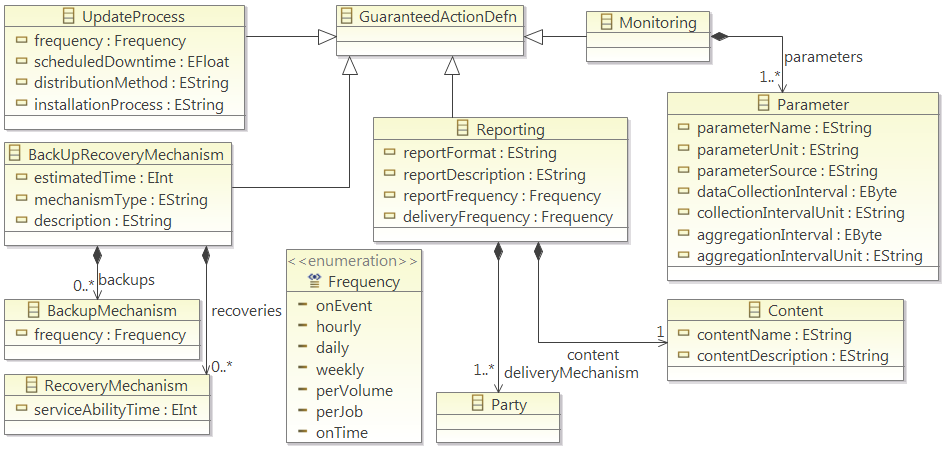
\includegraphics[width=0.75\textwidth]{fig/sloa_func_actions.png}
\end{center}
\caption{Business Level Guaranteed Action Classes}
\label{fig:business_level_garanteed}
\end{figure*}

\subsubsection{Business Level Guaranteed Actions}
The {\it Business Level Guaranteed Actions} has currently monitoring and reporting action implemented. The monitoring classes are expanded for the SLO-As. Also the attribute {\it ParameterSource} was added. This allows it, to recognize properties throu their names, data types and its source (UUID). Also frequencies for the definition of report, aggregation and acquisition intervals. the following frequency types are added:
\begin{itemize}
\item {\it onEvent} instead of an interval an event triggers the action
\item {\it onTime} a constant time stamp triggers the action
\item {\it perJob} the interval is defined by the runtime of a job
\item {\it perVolume} a concrete value trigger the action. For example 30GB disk space is full, or 1000 connections are open 
\end{itemize}
A major change is the relation to the class {\it Parameter}. This was changed to composition with {\it 1:n} relation, where {\it n} must be at least 1. This allows the declaration of multiple parameters and together with the source of the parameter ({\it SourceParameter}) it is possible to assign values of the  depended SLO-As.  

\subsubsection{Use Cases}\label{usecase}
To illustrate possible applications this section presents use cases and gives the corresponding sample implementations. Cloud computing hugely benefits of the self-serve principle, which underlies it. Therefore it is particular important to give customers the possibility to fill in the SLO templates with only a few steps and in an self-explanatory way. Three use cases will show the modelling possibilities of  SLA-A:
% Figure \ref{fig:gui} shows a sample GUI arrangement, where customers can select KPIs relevant to their needs and set the correspondig values. 
%
%\begin{figure}[ht]
%\includegraphics[width=0.5\textwidth]{fig/GUI.png}
%\caption{GUI for specifing customer SLOs}
%\label{fig:gui}
%\end{figure}

\subsubsection{Availability Use Case}
For the first use case we assume that a customer runs a cloud application on an specific regular basis. Therefore he wants to ensure that the resources are available for this specific times and can be used. We assume that the customer already has completed the initial process of creating a valid SLA with an provider for his service. The contract thereby covers the sepcific service times, in this case every friday from 14:00 to 18:00. This timeframe is therefore stored in the class {\it ServiceTime} as a {\it serviceTimePair}, where the key {\it startTime} has the value 14:00:00 and the key {\it endTime} has the value 18:00:00. Additionally another field is filled in where the {\it interval} is  set to {\it weekly} and {\it friday} is the value for the day so that all the defined agreements, for example the availability  or response time are legaly binding for this specific period.

Due to the changing business environment the customer now wants to change the SLA, because he needs the same service to be available on every wednesday from 09:00 to 14:00. Therefore the customer loads the existing SLA and adapts the {\it ServiceTime} so that the new requirements are met. The respecting changes to the XML files can be seen in figure \ref{fig:serviceTime}. In the real life the cutomer would change these settings by loading the already defined SLA into a tool with an graphical user interface like presented before and would simply change the the {\it ServiceTime} and generate the new SLA. This however requires that the newly choosen parameters are inside the limitations given by the provider. This validation is done automatic within the adjustment tool. If the validation succeeds the SLA gets signed online by both parties and is leagaly binding. In the case of mismatching customer demands and provider offerings the SLA can not be signed and a manual negotiation process has to be performed.

\begin{figure}[ht]
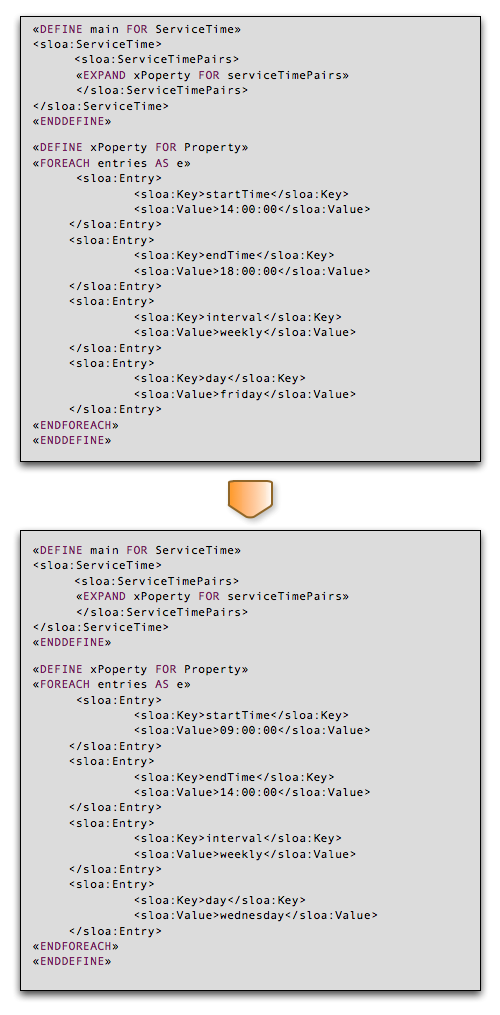
\includegraphics[width=0.5\textwidth]{fig/ServiceTimeChange.png}
\caption{serviceTime adjustment by the customer}
\label{fig:serviceTime}
\end{figure}


%% Abgleich mit Provider ?
%% Signing ?

\subsubsection{Additional KPI Use Case}
As exemplary second use case a customer wants to extend an existing SLA in order to match the advanced or varied requirements of his services, so the service quality can be better monitored and ensured. In this case the customer wants to add antother KPI, which represents his needs the best, to the existing SLA. For the SLA this means that another {it AgreementTerm} has to be added. Inside this {it AgreementTerm} the {it GuaranteedState}, it{GuaranteedAction}, etc. have to be specified. 
Additionally the {it ServiceLevelObjective} has to be created in order to measure and monitor the newly created KPI. If we assume that the customer wants to add the guarantee for the minimum bandwidth his service can use, this KPI and the corresponding {it interfaceDeclr} can be easiliy added by using the grapical interface like shown in figure ref{fig:gui}. Therefore the customer chooses a representing KPI from an list of available KPIs, fills in the appropriate values and so adds the new contract clause to the existing SLA. Again it has to be checked if newly added KPI is within the providers range of offerings or not and based on that can be signed online.
%%Beispiel XML file


% Kunde bucht zusätzliche Resource
\subsubsection{Additional Resource Use Case}
Another use case for using dynamic SLAs is to extend resources. For example, a customer wants to expand his computing power because of large and short term calculations. In this case the customer can order the new CPU power within the graphical interface, and he also is able to do that with time limitations. But it is necessary for the cloud provider to check the resources before he gives a garantuee to the customer for availability and pricing. 

\begin{figure}[ht]
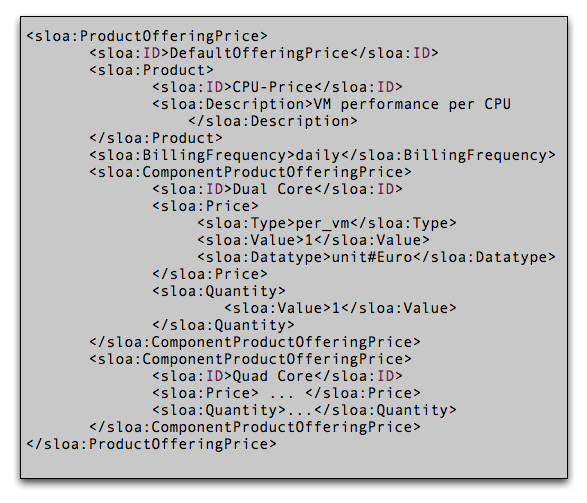
\includegraphics[width=0.5\textwidth]{fig/offering.png}
\caption{Service Offering for CPUs}
\label{fig:offering}
\end{figure}

For the pricing it is possible for the provider to give certain offers in regard of predefined bundles. In this way the provider is able to achieve a better resource allocation and usage prediction. A sample offering regarding the CPUs can be seen in figure ref{fig:offering}. There a special bundle price for dual core and quad core CPUs is given. The price is calculated by acumullating bundles. In special cases the customer can negotiate new terms with the provider. For the resource allocation the requested demand of the customer is checked against the real time resources of the provider. This is done automatically by inside the SLA creation tool. So after automatically checking the requested resources and calculating the new price the adjusted SLA is available for the customer and can be signed.


\section{QoS Management Modules}
\subsection{Threshold Value System}

\begin{figure}[ht]
	\centering
	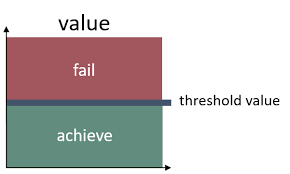
\includegraphics[width=0.7\linewidth]{chapters/chapter5/fig/threshold}
	\caption{}
	\label{fig:threshold}
\end{figure}

\subsection*{Fuzzy Inference }
Most approaches consider infrastructure sensor data like bandwidth, request/response time, CPU usage, memory usage, etc. to control the scaling infrastructure as depicted in Fig. \ref{fig:fuzzy_control_architecture} (dashed box). The approach of this paper is to use additional, often imprecise information (e.g. weather) to improve the management to meet the QoS requirements stated in SLAs. These imprecise factors (e.g. user wants scaling aggressive/moderate, etc.), political factors (legal changes, political summits, etc.), economic/market factors (product advertising, product launch, etc.), other factors influencing the service usage (e.g. weather, gossip, etc.) can not be modeled precisely.

Fuzzy logic allows to model imprecise information by the user in the form of non-numeric linguistic variables (e.g. weather: bad/good/excellent). These fuzzy inputs are used in the fuzzy control system, that uses expert knowledge to inference a fuzzy output. After defuzzifying this output to a crisp value, then this states how big the up and down scale factor should be. For example, if a customer wants to have an aggressive scaling control the infrastructure will scale up with e.g. 3 VMs otherwise with only one VM at a time. The scaling domain expertise is modeled in a knowledge base with fuzzy IF-THEN rules.

%In the next Subsection \ref{fuzzyScalingArchtecture} the architecture of the fuzzy scaling cloud service is described, followed by subsection \ref{fuzzyParameters}, discussing monitoring parameters, which will show a wide variety of information to improve the cloud scaling service. The last subsection \ref{fuzzyControlModule} presents the fuzzy control module.

\begin{figure}[ht]
\begin{center}
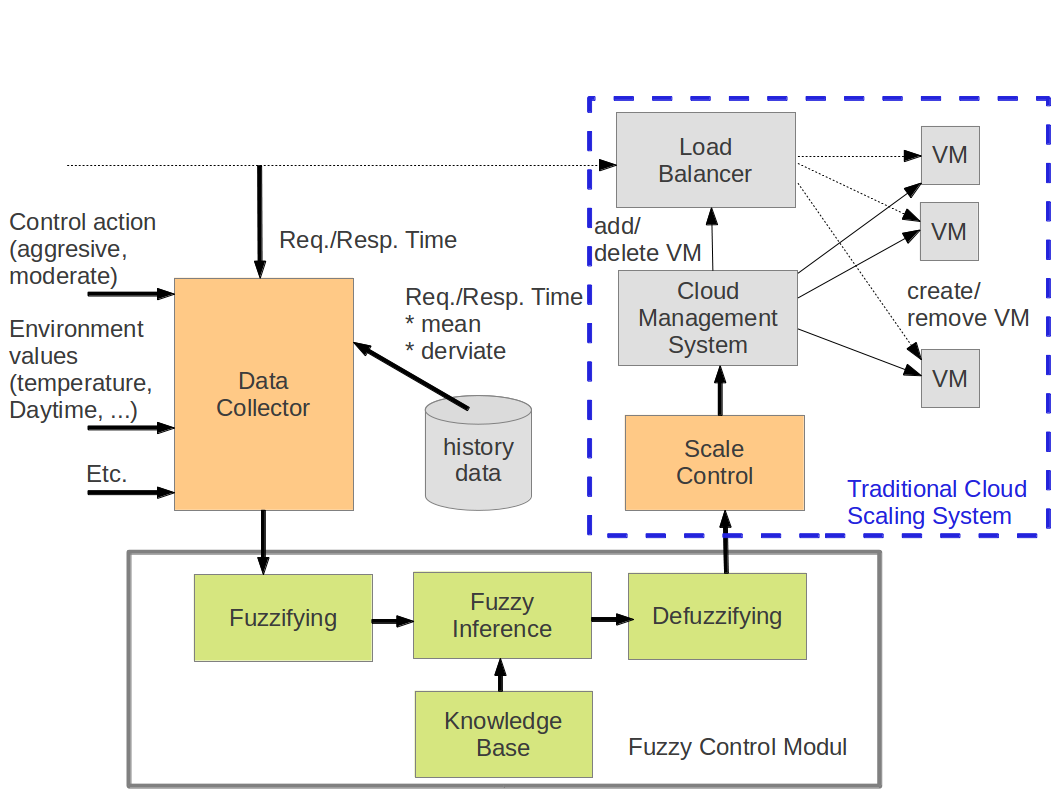
\includegraphics[width=0.5\textwidth]{fig/architecture}
\end{center}
\caption{Fuzzy Controlled Scaling Architecture}
\label{fig:fuzzy_control_architecture}
\end{figure}

\subsubsection{Fuzzy Controled Scaling Architecture}\label{fuzzyScalingArchtecture}
Figure \ref{fig:fuzzy_control_architecture} shows the architecture for a load balanced service by automatically scaling up/down the infrastructure by provisioning/deprovisioning VMs. It consists of two new modules compared to the traditional scaling infrastructure (blue box), the \textit{Data Collector} and the \textit{Fuzzy Control Module}.

The \textit{Data Collector} collects all information data, crisp (e.g. cpu usage) and imprecise data (e.g. weather). The data is categorized in infrastructure data (e.g. req./resp. time), history data (e.g. req./resp. time 5 minutes ago), control action (e.g. aggressive up/down scale), environment data (e.g. daytime), and other information that might influence the load of the service.  Some of the data is automatically monitored, like the infrastructure data, some is computed like the history data, and some is determined by users/experts like control action or environment data. 
All collected data is input data to the \textit{Fuzzy Control Module}, where the data is fuzzified, results are propagated by the fuzzy inference engine and quantified by defuzzification. The defuzzified value (Number of VM to be started or stopped) is put into the \textit{Scale Control} module, which generates XML-RPC calls to the \textit{Cloud Management System}.

\subsubsection{Collected Information Factors for the Fuzzy Control}\label{fuzzyParameters}
The relevant information to improve elasticity can be categorized into the following monitoring data: infrastructure, infrastructure history, time-dependent, and service-dependent sensor data. % described in the following paragraphs in more detail.

%\paragraph{Infrastructure Sensor Data}
%Table \ref{tab:InfrastructureSensorParameter}

Infrastructure sensor data includes factors that can mostly be monitored using sensors placed in various locations and layers of the cloud infrastructure. KPIs, like request response time, which can easily be measured at the load balancer (LB). Cloud specific parameters, like start time of VMs, can be aquisitioned at the cloud management system. % If user service request types should be categorized (typically a imprecise parameter), it is best to ask the user admin of the cloud resource.
%\begin{table}[ht]
%\caption{Infrastructure Sensor Parameter}
%\begin{center}
%\begin{tabular}{|l|l|l|}
%\hline
%Parameter & Example & Cloud Source\\
%\hline
%KPI & req./resp & load balancer\\
%\hdashline[.1pt/2pt]
%cloud specific & VM start time, & cloud management\\
%indicators & bandwidth & system\\
%\hdashline[.1pt/2pt]
%request type & long running req. & user\\
%\hdashline[.1pt/2pt]
%... & ... & ... \\
%\hline
%\end{tabular}
%\end{center}
%\label{tab:InfrastructureSensorParameter}
%\end{table}
The quality of the cloud infrastructure or service implementation can be taken into account as well. The load balancing control might be influenced by the basic robustness of the overall infrastructure. The infrastructure robustness can be modeled by an imprecise parameter e.g. strong, weak. 

%\paragraph{Infrastructure History Sensor Data}
%Table \ref{tab:HistoryInfrastructureSensorParameter} lists 
Infrastructure history sensor data are parameters that have been previously collected into a history data base. The purpose is to calculate values like, mean value, derivation value, etc. These statistical data can be good indicators to improve the LB management.
%\begin{table}[ht]
%\caption{Infrastructure History Sensor Parameter}
%\begin{center}
%\begin{tabular}{|l|l|l|}
%\hline
%Parameter & Example & Source\\
%\hline
%derivation KPI & derivation req./resp & history DB\\
%\hdashline[.1pt/2pt]
%mean value KPI & req./resp. mean value & history DB\\
%\hdashline[.1pt/2pt]
%... & ... & ...\\
%\hline
%\end{tabular}
%\end{center}
%\label{tab:HistoryInfrastructureSensorParameter}
%\end{table}
Imprecise history parameters can be of interest as well. Suppose a service depends on the weather condition (e.g. online shop for winter tires), then a sudden change of the weather condition from dry to snowy condition makes it more likely, that the load of such a service is higher.

%\paragraph{Time-Dependent Sensor Data}
%Table \ref{tab:TimeDependentSensorParameter} lists parameter that can influence the infrastructure management at a predefined time.
%\begin{table}[ht]
%\caption{Time-Dependent Sensor Parameter}
%\begin{center}
%\begin{tabular}{|l|l|l|}
%\hline
%Parameter & Example & Source\\
%\hline
%daytime & end of work & user input\\
%\hdashline[.1pt/2pt]
%weekday & Saturday & calendar\\
%\hdashline[.1pt/2pt]
%holiday & Christmas & country holiday cal.\\
%\hdashline[.1pt/2pt]
%product events & new iPhone & user input\\
%\hdashline[.1pt/2pt]
%... & ... & ...\\
%\hline
%\end{tabular}
%\end{center}
%\label{tab:TimeDependentSensorParameter}
%\end{table}
Time-dependent sensor data contain parameters that can influence the infrastructure management at a predefined time. The knowledge of the typical weekly usage for an service (see Fig. \ref{fig:weakload}) can be modeled and therefore the decision to scale up or down strongly or weakly depending whether the change is high or not.
\begin{figure}[ht]
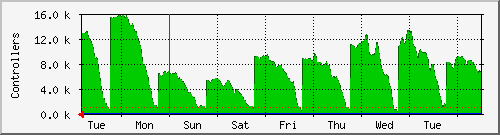
\includegraphics[width=0.45\textwidth]{fig/olat_week_usage}
\caption{Example: Weekly Load of the HFU Learning Management Platform}
\label{fig:weakload}
\end{figure}

%\paragraph{Service-Dependent Sensor Data}
%Table \ref{tab:ServiceDependentSensorParameter} 
Service-dependent sensor data involve parameters that influence the control infrastructure depending on the related service. Political parameters, like new legal issues enforcing more logging at the service side. Market events, like product launches, marketing events, new prices, etc. can influence the usage of services. Gossip, modeled as good news or bad news is influencing service usages. Importance of service might need a more aggressive management to make sure, that the SLA violations can be minimized.
%\begin{table}[ht]
%\caption{Service-Dependent Sensor Parameter}
%\begin{center}
%\begin{tabular}{|l|l|l|}
%\hline
%Parameter & Example & Source\\
%\hline
%politic & EU summit & news ticker\\
%\hdashline[.1pt/2pt]
%market price & Facebook share & exchange feed\\
%\hdashline[.1pt/2pt]
%gossip & new Facebook mobile & news ticker\\
%\hdashline[.1pt/2pt]
%service & control behavior & \\
%\hdashline[.1pt/2pt]
%importance & (moderate/aggressive) & user\\
%\hdashline[.1pt/2pt]
%... & ... & ...\\
%\hline
%\end{tabular}
%\end{center}
%\label{tab:ServiceDependentSensorParameter}
%\end{table}

\subsubsection{Fuzzy Control Module}\label{fuzzyControlModule}
The \textit{Fuzzy Control Module} consists of four main fuzzy control processes represented by the four sub-modules respectively (see Fig. \ref{fig:fuzzy_control_architecture}). The crisp and imprecise input data is converted into fuzzy values for each input fuzzy set with the \textit{Fuzzifying} module.
The decision making logic of the \textit{Fuzzy Inference} module determines how the fuzzy logic operations are performed (SUP-MIN inference), and together with the \textit{Knowledge Base} module determine the outputs of each fuzzy IF-THEN rules. Those are combined and converted to crisp values with the \textit{Defuzzification} module. The output crisp value can be calculated by the center of gravity or the weighted average and are converted to the number of VM to started or stopped.

\begin{figure}[ht]
\begin{center}
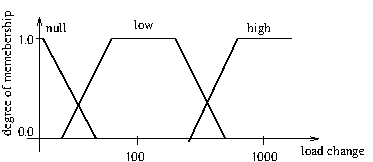
\includegraphics[width=0.35\textwidth]{fig/fuzzy_load_usage.png}
\end{center}
\caption{Input Fuzzy Set for Load Deviation}
\label{fig:fuzzy_inputset}
\end{figure}

\paragraph*{Fuzzification}
Fuzzification is the process of decomposing the input data into fuzzy sets, with trapezoidal shaped membership functions. Figure \ref{fig:fuzzy_inputset} shows a system of fuzzy sets for an input with trapezoidal membership functions. Any particular input is interpreted from this fuzzy set and a degree of membership is interpreted. If the request-response-time, for example, it set to about 100 request-per-seconds, the fuzzy value $load deviation$ is set to $low$.

\paragraph*{Fuzzy Inference}
The fuzzy values gathered from the input data are processed by the inference engine using the expert domain knowledge modeled as fuzzy IF-THEN rules. The following fuzzy rules are examples how to state the domain knowledge in the area of up and down scale control.
\begin{verbatim}
IF ReqRespTime_rising=high AND
   expected_ReqRespTime_rising=high AND
   product_launch=now AND
   ....
THEN
   up_scale=very high
...
\end{verbatim}

\paragraph*{Defuzzification}
After the fuzzy reasoning the resulting linguistic output variable (e.g. scale up = high) needs to be translated into a crisp value (e.g. number of VMs to be started or stopped at time). Defuzzification maps the output from the fuzzy domain back into the crisp domain. The most common defuzzification methods is the Center-of-Area (C-o-A) often referred to as Center-of-Gravity and is defined as follows:
\begin{equation}
x^{*} = \frac{\int \mu_{i}(x) x dx}{\int \mu_{i}(x) dx}
\end{equation}
where $x^{*}$ is the defuzzified output, $\mu_{i}(x)$ is the aggregated membership function and $x$ is the output variable. The C-o-A method calculates the area under the scaled membership functions and within the range of the output variable and afterwards calculates the geometric center of this area.


\subsubsection{Simulation Environment}\label{SimEnv}
In order to test the feasibility of our approach, we created a simulation environment to be capable of validating the general fuzzy controlled scaling architecture proposed in this paper. The simulator therefore consists out of four major modules (see Fig. \ref{fig:module_diagram}). Firstly, the \textit{request generator module}, which simulates the real life usage by generating requests to the cloud service. It is important to note, that in this simulation requests are generated with an static predefined workload trend. The second component is the \textit{load balancer module}, which distributes the generated requests equally to the pooled Virtual Machines (VMs) by ound-robin. Here also the request response time is determined, therefore the time from generating the request until the response arrives at load balancer is measured. Within the \textit{logic modules} this determined request response times then are checked and based on the stored fuzzy or conventional rules will be decided to scale the service up, down or do nothing.  And finally the \textit{scaler }, which connects to the actual cloud management system, which is responsible for the provision and adding or removal of resources. The used conventional rules are represented by an simple boundary system based with a low and high threshold. When the measured average request response hits the upper boundary a VM gets started or when the lower boundary is hit a VM is stopped. These boundary systems are widely used and provide a common way of QoS management.
\begin{figure}[ht]
\begin{center}
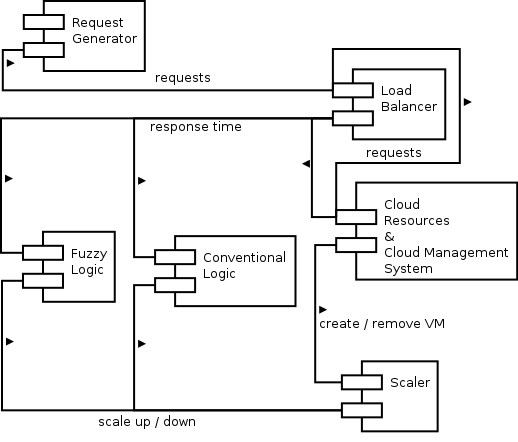
\includegraphics[width=0.38\textwidth]{fig/ModuleDiagram2.png}
\end{center}
\caption{Simulator Module Diagram}
\label{fig:module_diagram}
\end{figure}
The fuzzy set basically uses the same boundaries as the conventional rules, but as additional decision factors, an prediction based on expert knowledge or outlooks is used. This additional information allows an earlier respond to the changing loads and thus an better reaction to upcoming demands. Based on historical data the approximate usage and thus the load can be determined for a service. Figure \ref{fig:weakload} show the historic data of the load for an service during a week, based on this a simplified load prediction during daytime can be derived. %An simplified version of the expected service load during daytime is shown in Figure \ref{fig:daytimeload}.
%\begin{figure}[ht]
%\begin{center}
%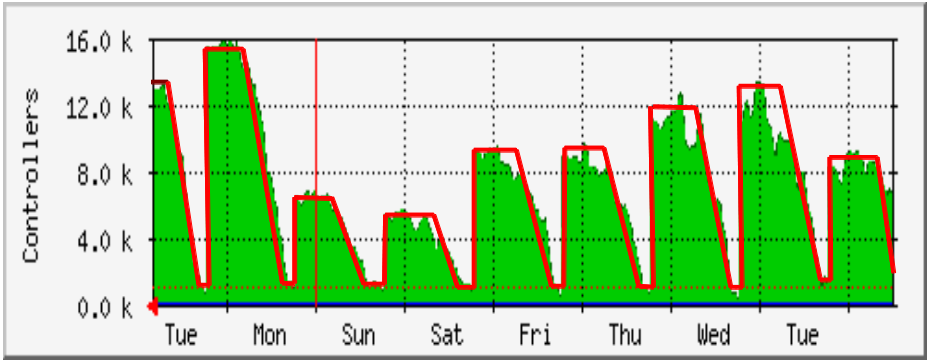
\includegraphics[width=0.35\textwidth]{fig/olat_week_usage_simplified.png}
%\end{center}
%\caption{Expected Service Load}
%\label{fig:daytimeload}
%\end{figure}

Based on such knowledge an expert specifies whether the load will expectedly be increasing at an high, regular or low rate. An predicted regular load will result in an rule set that equals the conventional boundaries,  therefore resulting in essentially the same behavior. In case of an high prediction, the scaler generally scales up faster, which means VMs are started on a lower load and additionally up to two VMs can be started at the same time based on the load. Simultaneously the scale down boundary is set to a lower load to keep a higher pool of available VMs. The low prediction, is in principle a reversed high prediction, which will change the behaviour into generally scale up later and scale down faster and up to two machines at once. 

As an additional basis for decision, the slope of the last measured points is used. The basis for this assumption is that a strong growth of response time indicates a upcoming peak load. The slope factor is therefore calculated of two response time values with the following formula:

\begin{equation}
slope_{a} = \frac{\Delta Y}{\Delta X} = \frac{Y_{2} -Y_{1}}{X_{2}-X_{1}}
\end{equation}

Where $ Y $ and $ X $ are the time and value of the measured response time and $slope_{a}$ is the currently determined slope. Since the course response time is unlikely linear, the slope must be determined more than once in order to reconstruct the actual system behaviour. Problematic are load bursts, which the determined slope suddenly rises or falls down extremely. In the worst case this could cause a VM to be started up and immediately get shut down again or vice versa. Therefore, the average of of the last $n$ slopes are used for the assessment. 
% \begin{figure}[ht]
% \begin{center}
% 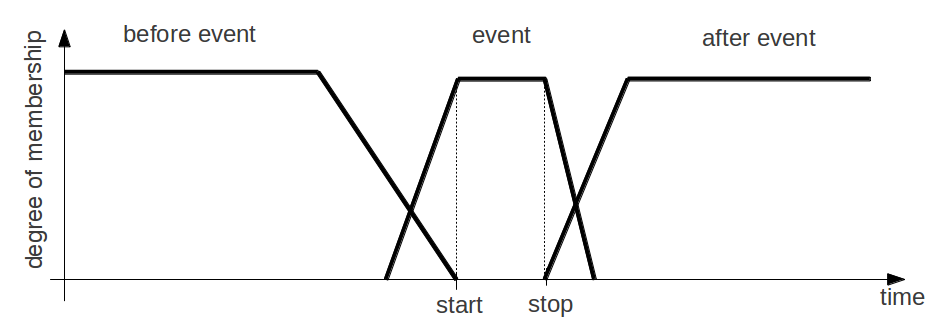
\includegraphics[width=0.45\textwidth]{fig/fuzzyevent.png}
% \end{center}
% \caption{Load Graph}
% \label{fig:fuzzyevent}
% \end{figure}
The simulator is based on a model in which a generated request includes a static processing time of 100ms. The KPI, is measured as the request/response time, based on the average of the last 10 processed requests. Thereby the time is counted form the generation of the request, till arrival of the response after the processing at the load balancer. The QoS limit has been set to 2000ms in this model and the conventional rule set regulates at an average response time of 1500ms by upscaling and at 1000ms by down scaling one VM at a time. To eliminate the influences of the test environment, like processor fluctuations the factor of 10 was used to all above described values.

%\begin{figure}[ht]
%\begin{center}
%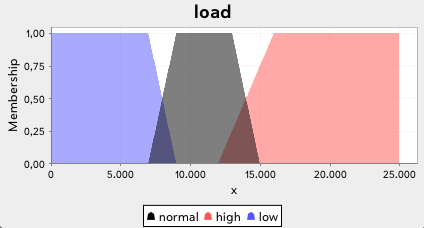
\includegraphics[width=0.45\textwidth]{fig/Fuzzy.png}
%\end{center}
%\caption{Responsetime Fuzzy Set}
%\label{fig:fuzzy_resp}
%\end{figure}
%Figure \ref{fig:fuzzy_resp} shows the corresponding fuzzy set, where a load of below 9,000ms is considered low and above 15,000ms is high. In between stretches the range of normal load. These fuzzy values are combined with the fuzzy prediction values to create the set of fuzzy rules.
To determine the suitability of the procedure presented, different scenarios have been created and tested with and without the fuzzy control mechanism. %Following the scenario with the specific preconditions and characteristics is described and the obtained results a presented. 
 
%\subsection{First Simulation Scenario}\label{SimScen} 
%In the first scenario the number of generated requests are increased rapidly and kept constant on a high level for an minute then rapidly decrease again. %Figure \ref{fig:s1load}  shows the corresponding load graph for this scenario. 
%This scenario simulates a classical peak load which happens when a service is facing an sudden demand, for example, accessing the canteen online menu just before the lunch break. Peak loads represent a problem in the real world, as countermeasures are most difficult. 
%
%%\begin{figure}[ht]
%%\begin{center}
%%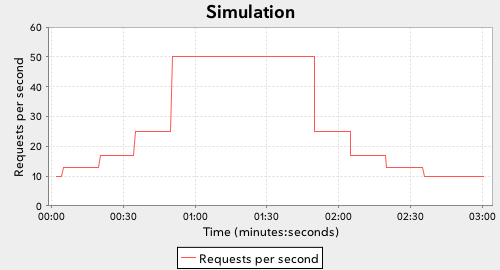
\includegraphics[width=0.45\textwidth]{fig/S1_Load.png}
%%\end{center}
%%\caption{Scenario 1: Load Graph}
%%\label{fig:s1load}
%%\end{figure}
%
%\textit{Result with conventional rule set:} The results for the simulation with the conventional rule set is shown in figure \ref{fig:s1conventional}. Obviously the maximum response time of 20.000ms is exceeded. This would mean that in the real world of the SLA violated. The simulation begins with the minimum of 2 VMs in the pool. In the first 35 seconds in the simulation the load is low enough for this two machines to cope with the requests. Afterwards the average response time starts rising slowly. At 50 seconds in the simulation the load gets increased even more. From this point, the response time increases sharply, until the first boundary limit of 15,000ms is hit and an additional VM gets started.
%
%\begin{figure}[ht]
%\begin{center}
%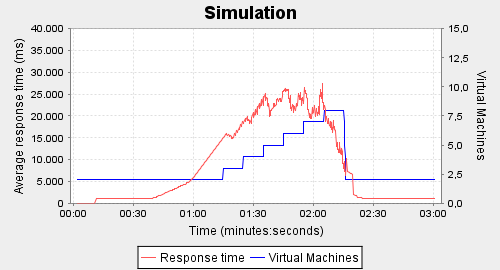
\includegraphics[width=0.45\textwidth]{fig/Testreihe1/01_normal.png}
%\end{center}
%\caption{Scenario 1: Conventional Rule Set Results}
%\label{fig:s1conventional}
%\end{figure}
%
%Since the conventional rule set can only start one VM at the same time, the system must wait until the VM has booted up only to realize that this is not enough to get the response time back within the desired range. So it starts one VM after another. Throughout the simulation up to 8 VMs are running simultaneously to manage the load. The large fluctuations seen at the peak of the load can be explained by the forming the average response time. The individual values between newly started and already longer running VMs vary widely because of the waiting time of the processing packets in the different VMs input queues.
%% nächster Satz verstehe ich nicht?
%A comparison with the fuzzy rule set and \textit{normal} prediction is not needed, since the results correspond due to the same rules.
%
%\begin{figure}[ht]
%\begin{center}
%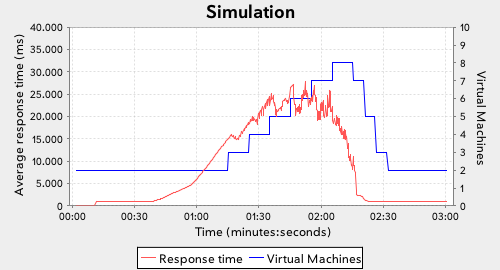
\includegraphics[width=0.45\textwidth]{fig/S1_Fuzzy_Low.png}
%\end{center}
%\caption{Scenario 1: Fuzzy \& "Low" Prediction Results}
%\label{fig:s1lowprediction}
%\end{figure}
%
%\textit{Result with fuzzy rule set (low prediction):} Comparing these results with the fuzzy rules with \textit{low} prediction as seen in figure \ref{fig:s1lowprediction}. It becomes clear that the results compared to conventional rule set are pretty similar. This is because with an low prediction, the limits for the up scale are unchanged and correspond to those of the conventional rules. Thus, in both the procedures the VMs are  added at the same load margins. The major difference occurs at the decreasing load, when shutting down the VMs. Here the fuzzy rules can shut down two VMs at once. This behavior has however no effect on the in this simulation already sinking response time, but it could save resources and money in real life situations. In both cases the QoS limit of 20,000ms is exceeded.
%
%\begin{figure}[ht]
%\begin{center}
%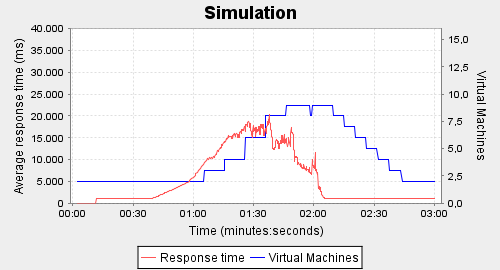
\includegraphics[width=0.45\textwidth]{fig/Testreihe1/03_prediction.png}
%\end{center}
%\caption{Scenario 1: Fuzzy \& "High" Prediction Results}
%\label{fig:s1highprediction}
%\end{figure}
%
%\textit{Result with fuzzy rule set (high prediction):} Figure \ref{fig:s1highprediction} shows the results for the simulation with the fuzzy rule set and \textit{high} prediction. In comparison to the other two results, this time the limit of 20,000 ms can be complied. In general this simulation produces a similar but shallower curve. Although this procedure uses the same maximum number of 8 VMs the achieved results in relation to the response time are much better. This can be attributed to the stronger up scale of starting two VMs simultaneously. This marginal difference is sufficient to prevent the response time from increasing over the QoS limit. The earlier intervention, which is already engaged at a normal load, prevents the requests from accumulating in the input queues of the VMs. Overall, though, more resources are used than in the previous tests. It must be decided whether the additional expenses through to additional resources are more economical the an SLA violation. This has to be decided by an expert and depends on the penalties specified in the SLAs.
%
%\begin{figure}[ht]
%\begin{center}
%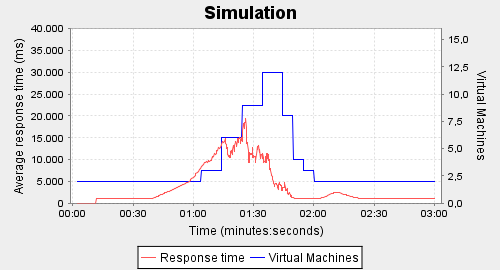
\includegraphics[width=0.45\textwidth]{fig/Testreihe1/04_slope.png}
%\end{center}
%\caption{Scenario 1: Fuzzy \& "High" Prediction \& Slope Results}
%\label{fig:s1slope}
%\end{figure}
%
%\textit{Result with fuzzy rule set (high prediction \& slope):} The fuzzy set with the additional decision factor slope allows to launch up to 5 VMs simultaneously. This  results in the use of an maximum of 11 VMs simultaneously. The result shows an further improvement in the form of an flatter curve. The highest value of the response time is less than that of the fuzzy rules with \textit{high} prediction. Therefore this regulation method is capable of shutting down the first VMs earlier then before, because not so many requests are stuck in the queues of the individual VMs. As an result, and by the fact that this regulation can disable up to 5 VMs at the same time, a lower resource usage profile is created, which could in reality lead to a lower overall price, as long as there are no additional costs for starting individual VMs.
%
%
%%Hier noch Bild von Fuzzy set für slope und erklärung für die anpassung auf allocation factor


\subsubsection{Simulation Scenario}\label{SimScen2}
In the presented scenario an complex course of load is sent to the service. In the first three minutes there is an peak demand, followed by reoccurring burst loads. This scenario simulates an peak load that doesn't  flatten quickly. This could be the case for services that depend heavily on news (e.g. launch of intensive product advertising). If the related service shows up in the news a initial large peak is produced and is recreated as smaller recurring peaks by spreading the word. Figure \ref{fig:s2load} shows load graph for this scenario.%This event is fuzzified by the following general membership function (see Fig. \ref{fig:fuzzyevent}. An event has a start and a end time. The fuzzy rule set basically state that during the event the number of VMs started is bigger then before or after the event.
%\begin{figure}[ht]
%\begin{center}
%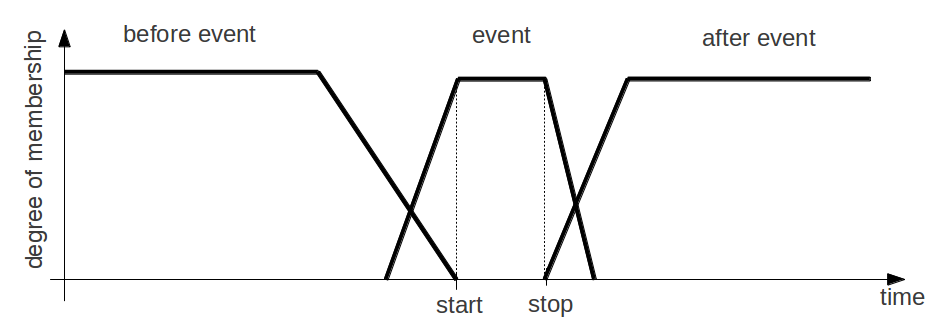
\includegraphics[width=0.45\textwidth]{fig/fuzzyevent.png}
%\end{center}
%\caption{Load Graph}
%\label{fig:fuzzyevent}
%\end{figure}

%Figure \ref{fig:s2load} below shows the correspondig graph for the load.
\begin{figure}[ht]
\begin{center}
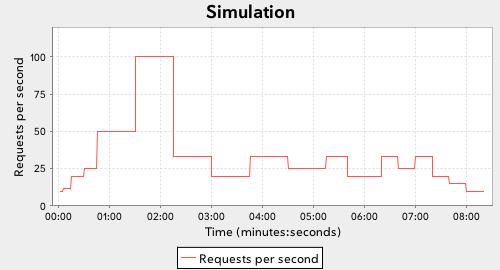
\includegraphics[width=0.40\textwidth]{fig/S2_Load.png}
\end{center}
\caption{Load Graph}
\label{fig:s2load}
\end{figure}

\textit{Result with conventional rule set:} The conventional rule set result graph shows that in this test the QoS limit of 20,000ms is exceeded for the first initial peak load and is nearly hit for the following rises. The scaling lags behind compared to the load increase. So it can not cope with the increasing load fast enough by starting new VMs. 
\begin{figure}[ht]
\begin{center}
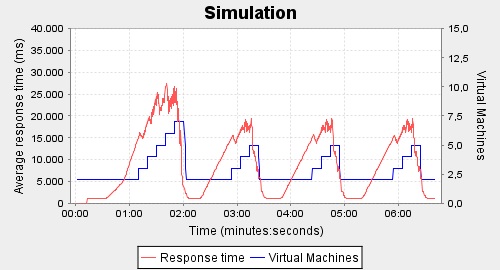
\includegraphics[width=0.40\textwidth]{fig/Testreihe2/01_normal.png}
\end{center}
\caption{Conventional Rule Set Results}
\label{fig:s2normal}
\end{figure}
This is clearly proven by the fact that the maximum number of VMs simultaneously used is only reached immediately before the flattening of the load.  
 
\textit{Result with fuzzy rule set (high prediction):} Compared to output of the fuzzy rules with \textit{high} prediction, as shown in figure \ref{fig:s2high}, it becomes clear that here the VMs are much earlier for disposal allowing to reduce the response time and be inside the SLA margin. Although for the first peak load two VMs additional VMs are used, this resembles a relatively small expense in compare to breaking the SLA. It is shown later on in the simulation that better results are delivered in the smaller peaks with the same number of VMs.

\begin{figure}[ht]
\begin{center}
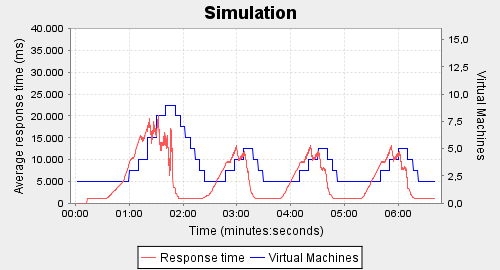
\includegraphics[width=0.40\textwidth]{fig/Testreihe2/03_prediction.png}
\end{center}
\caption{Fuzzy \& "High" Prediction Results}
\label{fig:s2high}
\end{figure}
\textit{Result with fuzzy rule set (high prediction \& slope):} Comparing these results with those of the fuzzy rules with \textit{high} prediction and \textit{slope} (see Figure \ref{fig:s2slope}), the response time has been reduced again, in spite of the very rapid scale up of VMs. The response time is in the range of all other peaks and is in this case is maintained very spacious. However, in this case an additional VM is switched on compared to the fuzzy rules with \textit{high} prediction. The large differences in the results graphs are however not  dependent on this additional resource. Instead the upscaling of several VMs simultaneously achieves the improvement. In this case it is up to 3  VMs are allocated at the same time.


\begin{figure}[ht]
\begin{center}
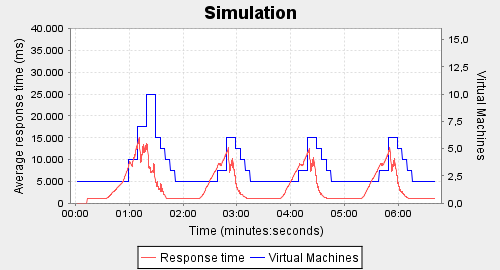
\includegraphics[width=0.40\textwidth]{fig/Testreihe2/04_slope.png}
\end{center}
\caption{Fuzzy \& "High" Prediction \& Slope Results}
\label{fig:s2slope}
\end{figure}
It can be concluded that with the presented approach it is clear that more resources are used which can lead to higher costs for the customer. But the response time and the SLA thresholds are maintained better and less SLA violations occur. Whether this is economically in each case must be decided by experts contemplating the SLA and contract data.

\subsection{Machine Learning Algorithms}
To improve the output of the QoS Management Module, different machine learning algorithms were used to test the feasibility of the approach. Firstly a general Artificial Neural Network was used to predict different enviornmentall KPIs. Afterwards an investigation and comparison of Support Vector Machines, Artificial Neural Network, and general Linear Regression was conducted.

\subsubsection{Artificial Neural Network}
Artificial neural networks, in short: ANN, are networks of artificial neurons which aims to simulate the process inside the human brain and represent a branch of artificial intelligence. Artificial neural networks have been successfully used in the past with all sorts of optimization problems, which makes them a suitabel approach for our solution. The aim of this first approach  was to create a prototype application which enables efficient provisioning of cloud storage resources with the use of Artificial Neural Networks to achieve better compliance with SLAs. The most common type of ANNs used for forecasting is the feedforward multilayer perceptron (ffMLP), as seen in Figure \ref{fig:Netz}. 

\begin{figure}[ht]
	\begin{center}
		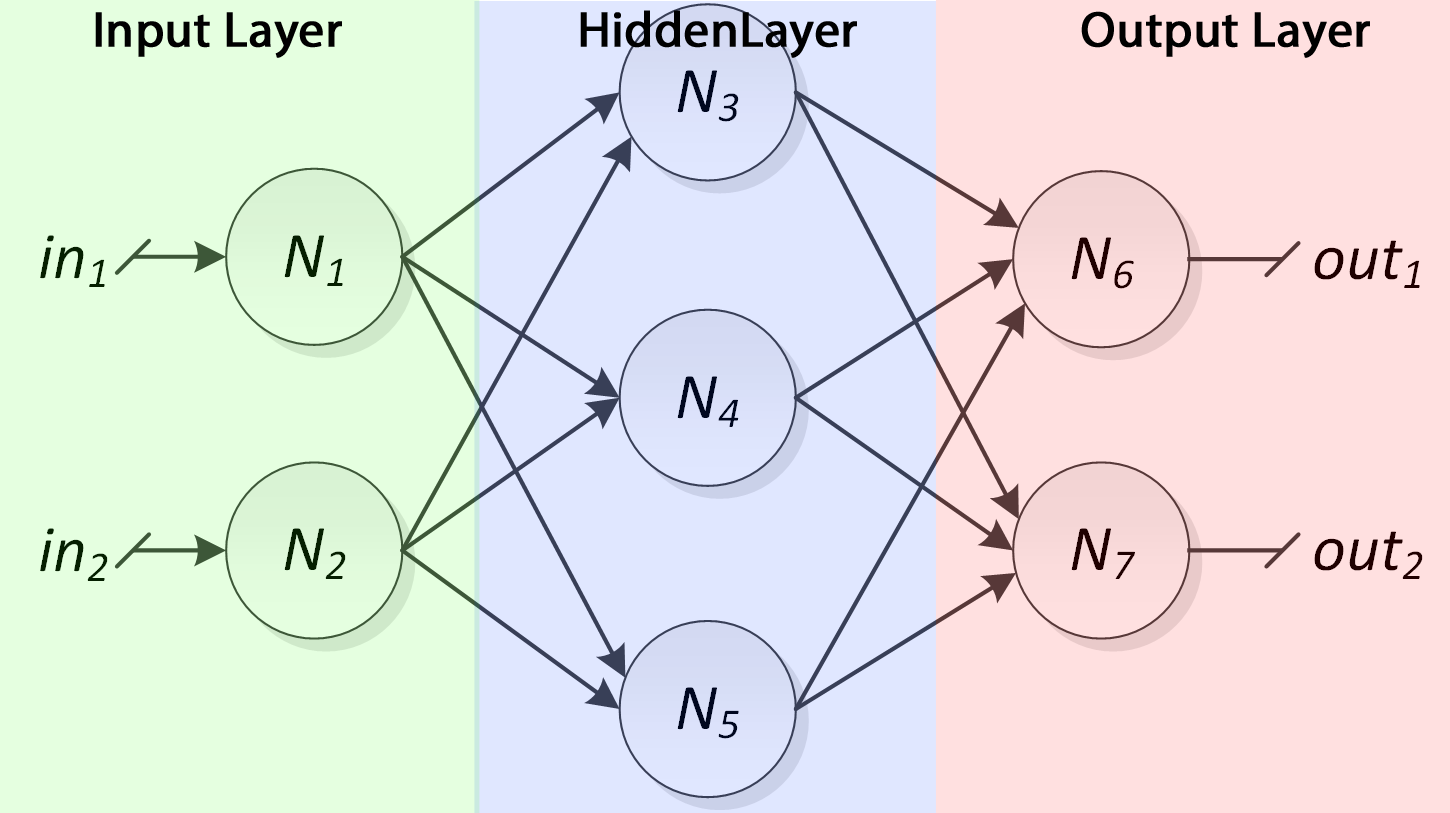
\includegraphics[width=0.45\textwidth]{fig/netz.png}
	\end{center}
	\caption{Simple 3-tier Feedforward Multilayer Perceptron.}
	\label{fig:Netz}
\end{figure}

These are Neural Networks, which consist of one input layer, $n$-hidden processing layers and one output layer. Feedforward networks are classified by each neuron in one layer having only direct connections to the neurons of the next layer, which means they have no feedback. In feedforward multilayer perceptrons, a neuron is often connected to all neurons of the next layer, which is called completely linked. So, there is no direct or indirect connection path from neuron $ N_{x} $ which leads back to a neuron $ N_{x-z} $. To compute a one-step-ahead forecast, these NNs are using lagged observations inputs of time series or other explanatory variables. 

For the creation of the Neural Network model we used the graphical editor and simulator MemBrain \cite{MemBrain}. The presented Neural Network consists of 119 neurons, which are aligned into 5 layers, and corresponds to a ffMLP where not all neurons are completely linked. An architectural overview of the presented model is shown in Figure \ref{fig:Netz2} below.


\begin{figure}[ht]
	\begin{center}
		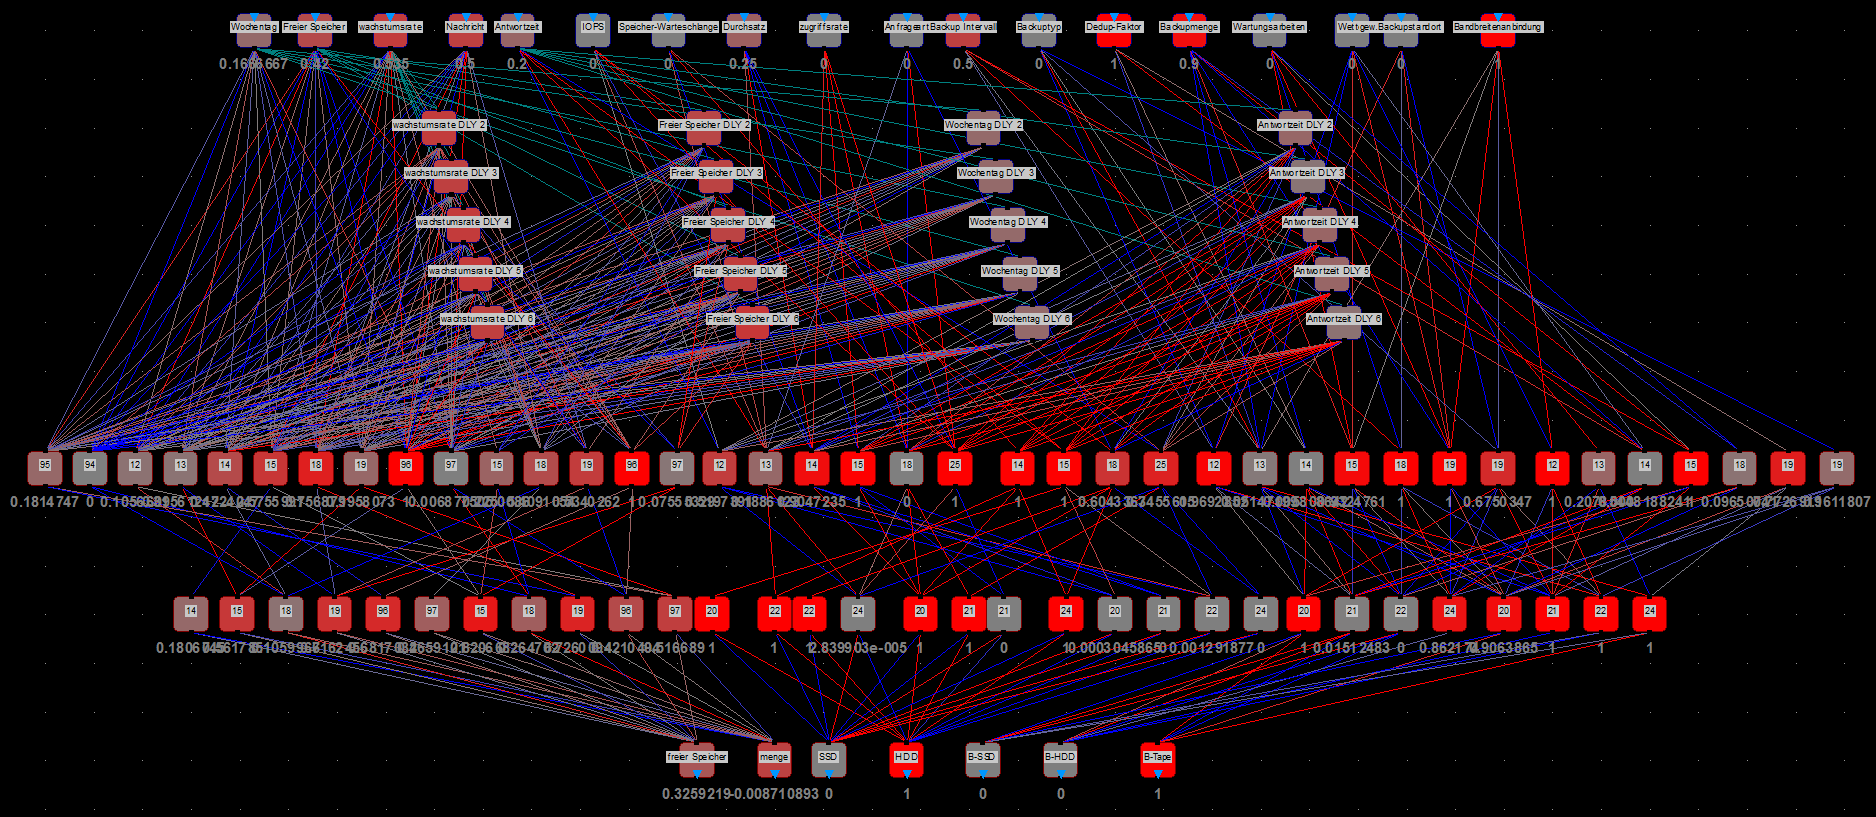
\includegraphics[width=0.48\textwidth]{fig/netz2.png}
	\end{center}
	\caption{Feedforward Multilayer Perceptron Architecture.}
	\label{fig:Netz2}
\end{figure}

Training of ANNs can be seen as a complex nonlinear optimization problem, and sometimes the network can  get trapped into a local minimum. ANNs can theoretically learn by developing new or deleting existing connections, changing the connection weights or threshold values, altering one or more of the three neuron functions (activation, propagation and output) and developing new or deleting existing neurons. In order to improve outputs, the input neurons should get normalized variables. This can simply be done by the equation below.
\begin{eqnarray}
X_{norm}  = \frac{X - X_{min}}{X_{max} - X_{min} }
\end{eqnarray}
In order to avoid local minima and bad results, the training should be initialized several times with different  starting weights and alignments. For the training of the proposed model, data sets were created in the form of Comma Separated Value (CSV) files. Each file contains storage usage patters with input and output vectors. Here, 60\% of the samples were used for training and the remaining 40\% were used for the validation of the network. The output behavior was modeled by depending on a input vector, where the desired output values where manually entered into the input vector. Thus, situations in which the responsible output neuron shall increase the amount of allocated memory were mapped.

To teach the network the prediction capability of future memory usage, the input vector was extended. The entire course of the used memory amount was added for the period of $ t_{0} $ to $ t_{n} $.  The desired output for this input vector at the given time $ t_{i} $ shall be the predicted amount of memory used at time $ t_{i + x} $. To achieve this, the value of the output vector at any point $ t_{i} $ in the time period $ t_{0} $ to $ t_{n} $ was set to the input vector of the point $ t_{i+x} $, by which $ x $ determines the length of the forecast period. Through this shift in values ​​the network can be trained for a prognosis. During each training session the network error was checked with validation data. MemBrain calculates this using the following formula: \begin{eqnarray}
NetError = \frac{\sum\limits_{i=1}^n{(Target_{i} - Output_{i})^2}}{n}
\end{eqnarray}
The desired activation of the output neurons is here referred to as $ Target $ and the actual calculated activation is the $ Output $. The squared deviations are summed and divided by the number of training data sets. To determine whether the Neural Network shows good results of the output behavior, it has been trained and validated with 10 different training data sets. The result for the network error after each learning processes is shown in Table \ref{tab:NetzFehler} below.

\begin{table}[ht]
	\caption{INFRASTRUCTURE SENSOR PARAMETER.}
	\begin{center}
		\begin{tabular}{|l|l|l|}
			\hline
			Training \newline Nr. & NetError \newline (Training) & NetError \newline (Validation)\\
			\hline
			1 & 0,0000573 & 0,046 \\
			\hdashline[.2pt/2pt]
			2 & 0,0000586 & 0,040 \\
			\hdashline[.2pt/2pt]
			3 & 0,0000713 & 0,040 \\
			\hdashline[.2pt/2pt]
			4 & 0,0000702 & 0,112\\
			\hdashline[.2pt/2pt]
			5 & 0,0000611 & 0,040 \\
			\hdashline[.2pt/2pt]
			6 & 0,0000783 & 0,083 \\
			\hdashline[.2pt/2pt]
			7 & 0,0000703 & 0,046 \\
			\hdashline[.2pt/2pt]
			8 & 0,0000627 & 0,038 \\
			\hdashline[.2pt/2pt]
			9 & 0,0000645 & 0,061 \\
			\hdashline[.2pt/2pt]
			10  & 0,0000630 & 0,046 \\
			\hline
		\end{tabular}
	\end{center}
	\label{tab:NetzFehler}
\end{table}
Here, it can be seen that the NetError reaches overall good values close to zero and not only for a particular dataset. The average total error for all training runs from Table \ref{tab:NetzFehler} is 0.0000657 for trained and 0.0573 for untrained (unknown) input data. 

\paragraph*{Evaluation}
The aim of this prototype was to investigate, whether or not the use of a Artificial Neural Network for the provisioning of a cloud storage resources has a positive effect on SLAs compliance, and whether this can lead to a better resource utilization compared to a classic threshold value system. For this purpose we created a simulation environment where storage requests (read, write, and delete) form a generator were sent trough a QoS monitor. Inside the QoS control module, the Artificial Neural Network and the threshold value system were used to regulate the amount of allocated storage capacity. Figure \ref{fig:arch} shows the architectural overview of the simulation environment.

\begin{figure}[ht]
	\begin{center}
		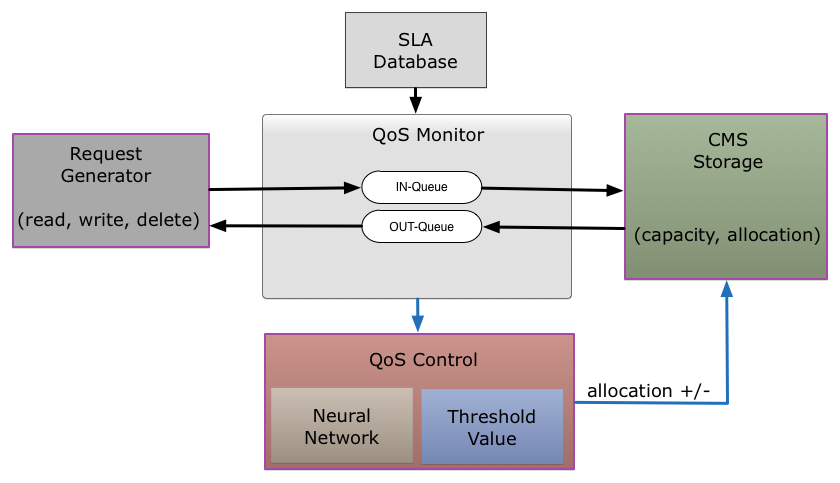
\includegraphics[width=0.5\textwidth]{fig/archi.png}
	\end{center}
	\caption{Simulation Architecture.}
	\label{fig:arch}
\end{figure}

In the simulation, the impact of regulatory mechanisms on the following key performance indicators was considered:
\begin{itemize}
	\item Free memory amount: providing an optimal amount of memory by the control logic. 
	\item Response time: compliance with the KPI response time by adjusting the storage medium. 
	\item Backup Media: proposal of a suitable backup medium.
\end{itemize}
For this, the used Neural Network consisted of  11 different input neurons. Table \ref{tab:input} lists the used input neurons and describes the used input factors. As output neurons, there is one neuron that gives the expected used memory amount for the next simulation step, a neuron that determines the amount of memory to be added or removed, as well as other neurons that recommend the optimal backup medium.

\begin{table}[ht]
	\caption{SIMULATION INPUT NEURONS}
	\begin{center}
		\begin{tabular}{|l|l|}
			\hline
			Neuron & Description\\
			\hline
			Time & Point $ t_{i}  $ in $ t_{0} ... t_{n} $ \\
			\hdashline[.2pt/2pt]
			Weekday  & Day of week for point $ t_{i}  $ \\
			\hdashline[.2pt/2pt]    
			Free Storage Capacity & Free storage capacity at point $ t_{i}  $\\
			\hdashline[.2pt/2pt]
			Growth Rate & Change of capacity from $ t_{i-1}  $ to $ t_{i}  $\\
			\hdashline[.2pt/2pt]
			Response time &  Mean response of last 5 inputs $ \frac{\sum_{i=i-5}^{i} t_i}{n}$\\
			\hdashline[.2pt/2pt]
			Queue Length  & Still open request at point $ t_{i}  $ \\
			\hdashline[.2pt/2pt]
			Troughput &  Troughput at point $ t_{i}  $ \\
			\hdashline[.2pt/2pt]
			Access Rate& Amount of requests per time slot \\
			\hdashline[.2pt/2pt]
			Request Type & Distinction between large and small requests\\
			\hdashline[.2pt/2pt]
			Backup Amount &  Size of backup data\\
			\hdashline[.2pt/2pt]
			Bandwidth & Usable bandwidth at point $ t_{i}$  \\
			\hline
		\end{tabular}
	\end{center}
	\label{tab:input}
\end{table}

In order to compare the results of the Neural Network with a common, in practice widely used method, a threshold value based scaling was implemented. This regulation system is controlled by predefined thresholds for the monitored KPI values. The implementation for the threshold rules for adding and removing allocated storage can be seen below in Figure \ref{fig:listing}, as simple pseudocode if then rules.
\\

\begin{figure}[ht]
	\begin{center}
		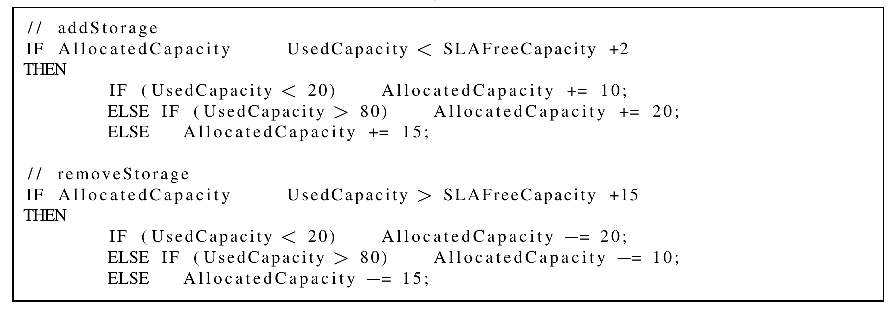
\includegraphics[width=0.5\textwidth]{fig/listing.png}
	\end{center}
	\caption{IF THEN rules for threshold system.}
	\label{fig:listing}
\end{figure}

%\tiny\begin{lstlisting}[caption = IF THEN Rules, frame=single] 
%// addStorage
%IF AllocatedCapacity − UsedCapacity < SLAFreeCapacity +2
%THEN
%  	IF (UsedCapacity < 20)    AllocatedCapacity += 10;
%	ELSE IF (UsedCapacity > 80)    AllocatedCapacity += 20;
%	ELSE   AllocatedCapacity += 15;
%	
%// removeStorage
%IF AllocatedCapacity − UsedCapacity > SLAFreeCapacity +15
%THEN
%  	IF (UsedCapacity < 20)    AllocatedCapacity -= 20;
%	ELSE IF (UsedCapacity > 80)    AllocatedCapacity -= 10;
%	ELSE   AllocatedCapacity -= 15;
%\end{lstlisting}
%\normalsize

Here, it can be seen that, by falling below a 2\% buffer of the storage value defined in the SLA, the allocation will be increased and by exceeding 15\% over the amount of storage defined in the SLA, the allocation will be lowered. The amount of which the allocated storage will be changed is dependent on how much the overall storage usage is. In case of an usage of over 80 \%) increase will be 20\%, with an usage of below 20\% the increase will be 10\% and in between the increase is 15 \% of the overall volume. These settings are reversed for the deallocation of the storage.

For the scenario in this simulation, a dynamic storage SLA, in which a customer gets granted 10GB of free space and up to 100GB of overall usage, was assumed. With such a dynamic limit described in the SLA, it is particularly important for the provider to find a solution that is as close as possible to the guaranteed amount of storage, since this will ensure a high economic efficiency. In practice, however, this usually is not possible. For this reason and because a violation of the SLAs can have monetary consequences, bigger buffer zones are installed. Figure \ref{fig:ResultsSW} shows the resulting graph of the simulation with the conventional threshold value rules.

\begin{figure}[ht]
	\begin{center}
		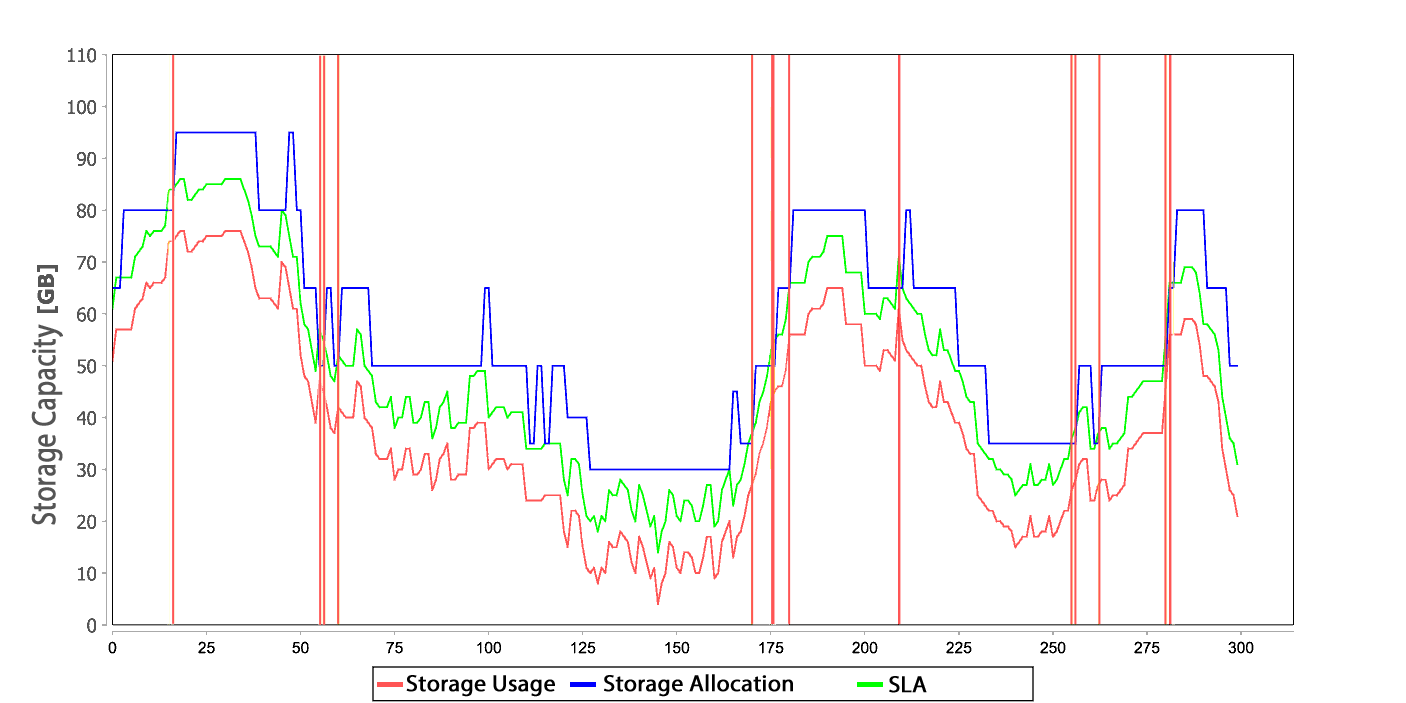
\includegraphics[width=0.5\textwidth]{fig/storage-sw2.png}
	\end{center}
	\caption{Storage allocation results for threshold rules.}
	\label{fig:ResultsSW}
\end{figure}

The red graph in Figure 5 and Figure 6 shows the course of the memory usage in GB, by the user during the simulation. The usage has been pre-generated for the simulation purpose and shall resemble a system, where a user regularly creates and deletes files with up to 15GB size, as well as generate larger files with up to 50GB. This type of usage may occur while working with different media files, like in the post-processing of movie projects. The green line marks the guaranteed amount of storage available to the user, granted by the SLA. It proceeds synchronous to the red graph, since the user gets guaranteed 10GB more than they currently use. The blue graph shows the pre-allocated amount of storage, which is directly usable by the user.

If we compare these results with those obtained by the Neural Network controlled storage allocation, shown in Figure \ref{fig:ResultsNN}, it becomes clear that the efficiency is marginally improved. With an average of 18.68\% of memory over provisioned the threshold value system is almost as effective as the neural network, with a 18.22\% overhead. The slight difference arises from the fact that the allocation offered by constantly adopting, fits to the SLA limits with a relatively constant overhead. In contrast, the threshold value system initially provides too much memory, and then only adopts the amount of allocated storage shortly before a violation of the SLA it to occur.

While comparing the two graphs, we see that the threshold system due to the fixed thresholds less often adjusts the amount of memory (blue curve). Since the added / removed amount of memory operates with a fixed predefined value​​, often too much memory is provided and then immediately gets removed again. This happens likewise when reducing the amount of memory allocated, which often leads to falling below the specified minimum amount in the SLA. However, the Neural Network determines constantly, based on the learned training data, a variable amount of memory that is to be added or removed, which leads to adequate reactions and a slightly better economic result.

\begin{figure}[ht]
	\begin{center}
		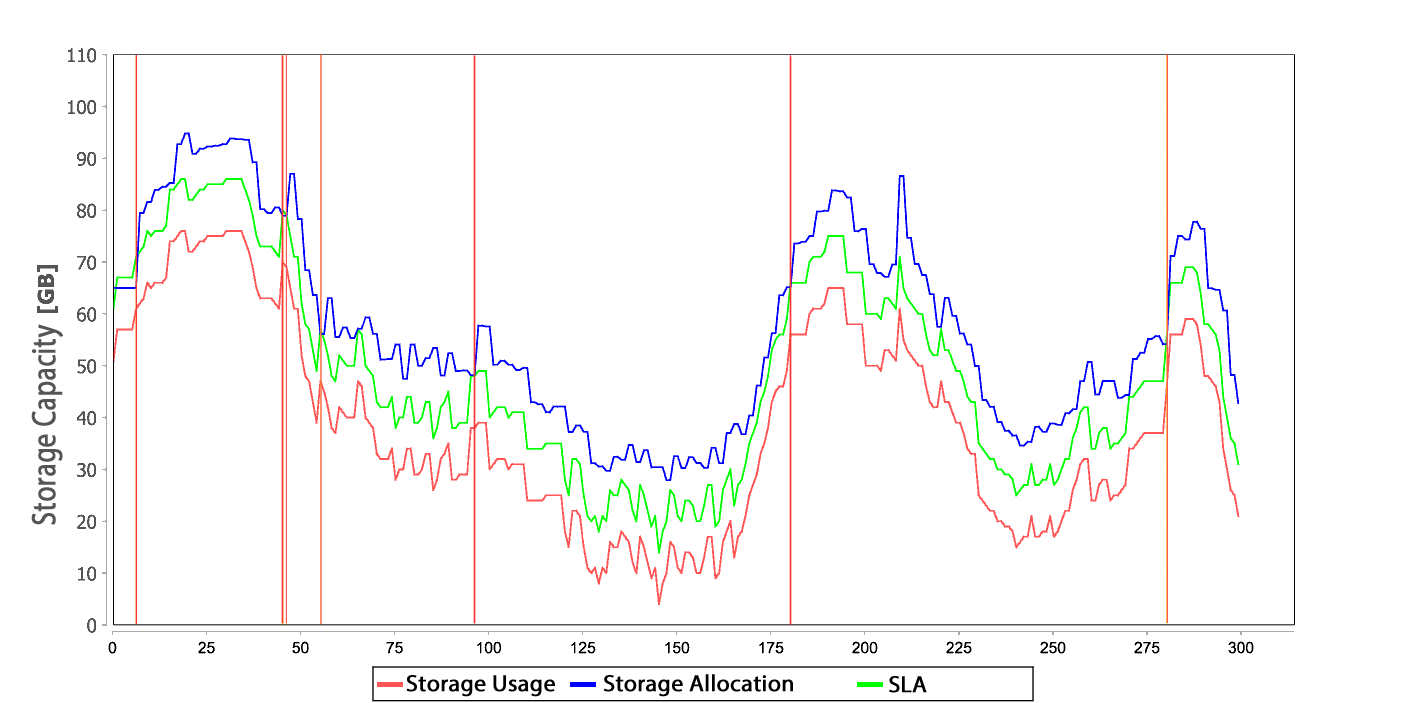
\includegraphics[width=0.5\textwidth]{fig/storage-nn3.png}
	\end{center}
	\caption{Storage allocation results for NN.}
	\label{fig:ResultsNN}
\end{figure}

However, when comparing the number of SLA violations, it becomes clear that the Neural Network approach delivers a significantly better solution. This is also evident in the resulted graph seen in Figures \ref{fig:ResultsNN} and \ref{fig:ResultsSW}, where the SLA violations are indicated by vertical red lines. These exemplary results of the simulation show that the Neural Network produces 7 and the threshold value system 13 SLA violations. These results were also confirmed within the other test runs, where the Neural Network generates an average of 7.45 violations per run and the threshold values system of 15.03 SLA violations per run. Overall, the Neural Network generated solution for the provisioning of storage is better suited, since the number of SLA violations is significantly lower. Together with the slightly lower overhead makes this a reasonably good solution.



\subsubsection{Support Vector Machines}\label{SVM}







\subsubsection{Evaluation}\label{MLeval}
In order to apply and evaluate different Machine Learning algorithms, the open source software RapidMiner \cite{rapidminer} was used. The log files created by the CloudSim application were utilized as training and test sets. Furthermore, the available Series extension provided by RapidMiner was used. This extension enables an efficient way to quickly replace different Machine Learning algorithms during the process of creating and evaluating a model in regard to ordered time series.

With the help of a horizon of h=20 (2 seconds), it was defined that the learning algorithms gets to learn the next h time steps in order to be able to predict the value of the average response time of h+1. After the prediction, the time window is incremented by 1 and the next value gets predicted. 

\begin{itemize}
\item \textbf{Neural Network:} Feed forward NN, training back propagation | Hidden layers: 8 | Training cycles: 1000 | Learning rate: 0.3 | Momentum: 0.2 | Decay: true | Normalize: true | Error epsilon: 0.00001
\item \textbf{Support Vector Machines:} Kernel Type: radial | Kernel Gamma: 1.0 | Kernel cache: 200 | C: 0 | Convergence epsilon: 001 | Max iterations: 10000 | Scale: true | L pos: 1.0 | L neg: 1.0 3) Linear Regression: | Feature selection: Iterative T-Test |Max iterations: 1.0 | Forward alpha: 0.05 | backward alpha: 0.05 | eliminate colinear features: true | min tolerance: 0.05 | use bias: true 
\item \textbf{Linear Regression:} Feature selection: Iterative T-Test | Max iterations: 1.0 | Forward alpha: 0.05 | backward alpha: 0.05 | eliminate colinear features: true | min tolerance: 0.05 | use bias: true 
\end{itemize}


\paragraph*{Scenario 1}
The first testing scenario resembles a classical burst load. Here the server is hit with short bursts of high demand. In out test the requests at the server are highly increased during 10 seconds followed by a phase of low requests. This pattern ist repeated four times during the course of this test. This type of load can occur, for example, on servers that are attacked by botnet (denial of service attack). Alternatively, this pattern can also occur with automated access to APIs or synchronized access to data. In reality, this kind of load is particularly difficult to process since you can adjust it badly and depending on the scale used the system simply can be too slow.


\begin{figure}[ht]
	\begin{center}
		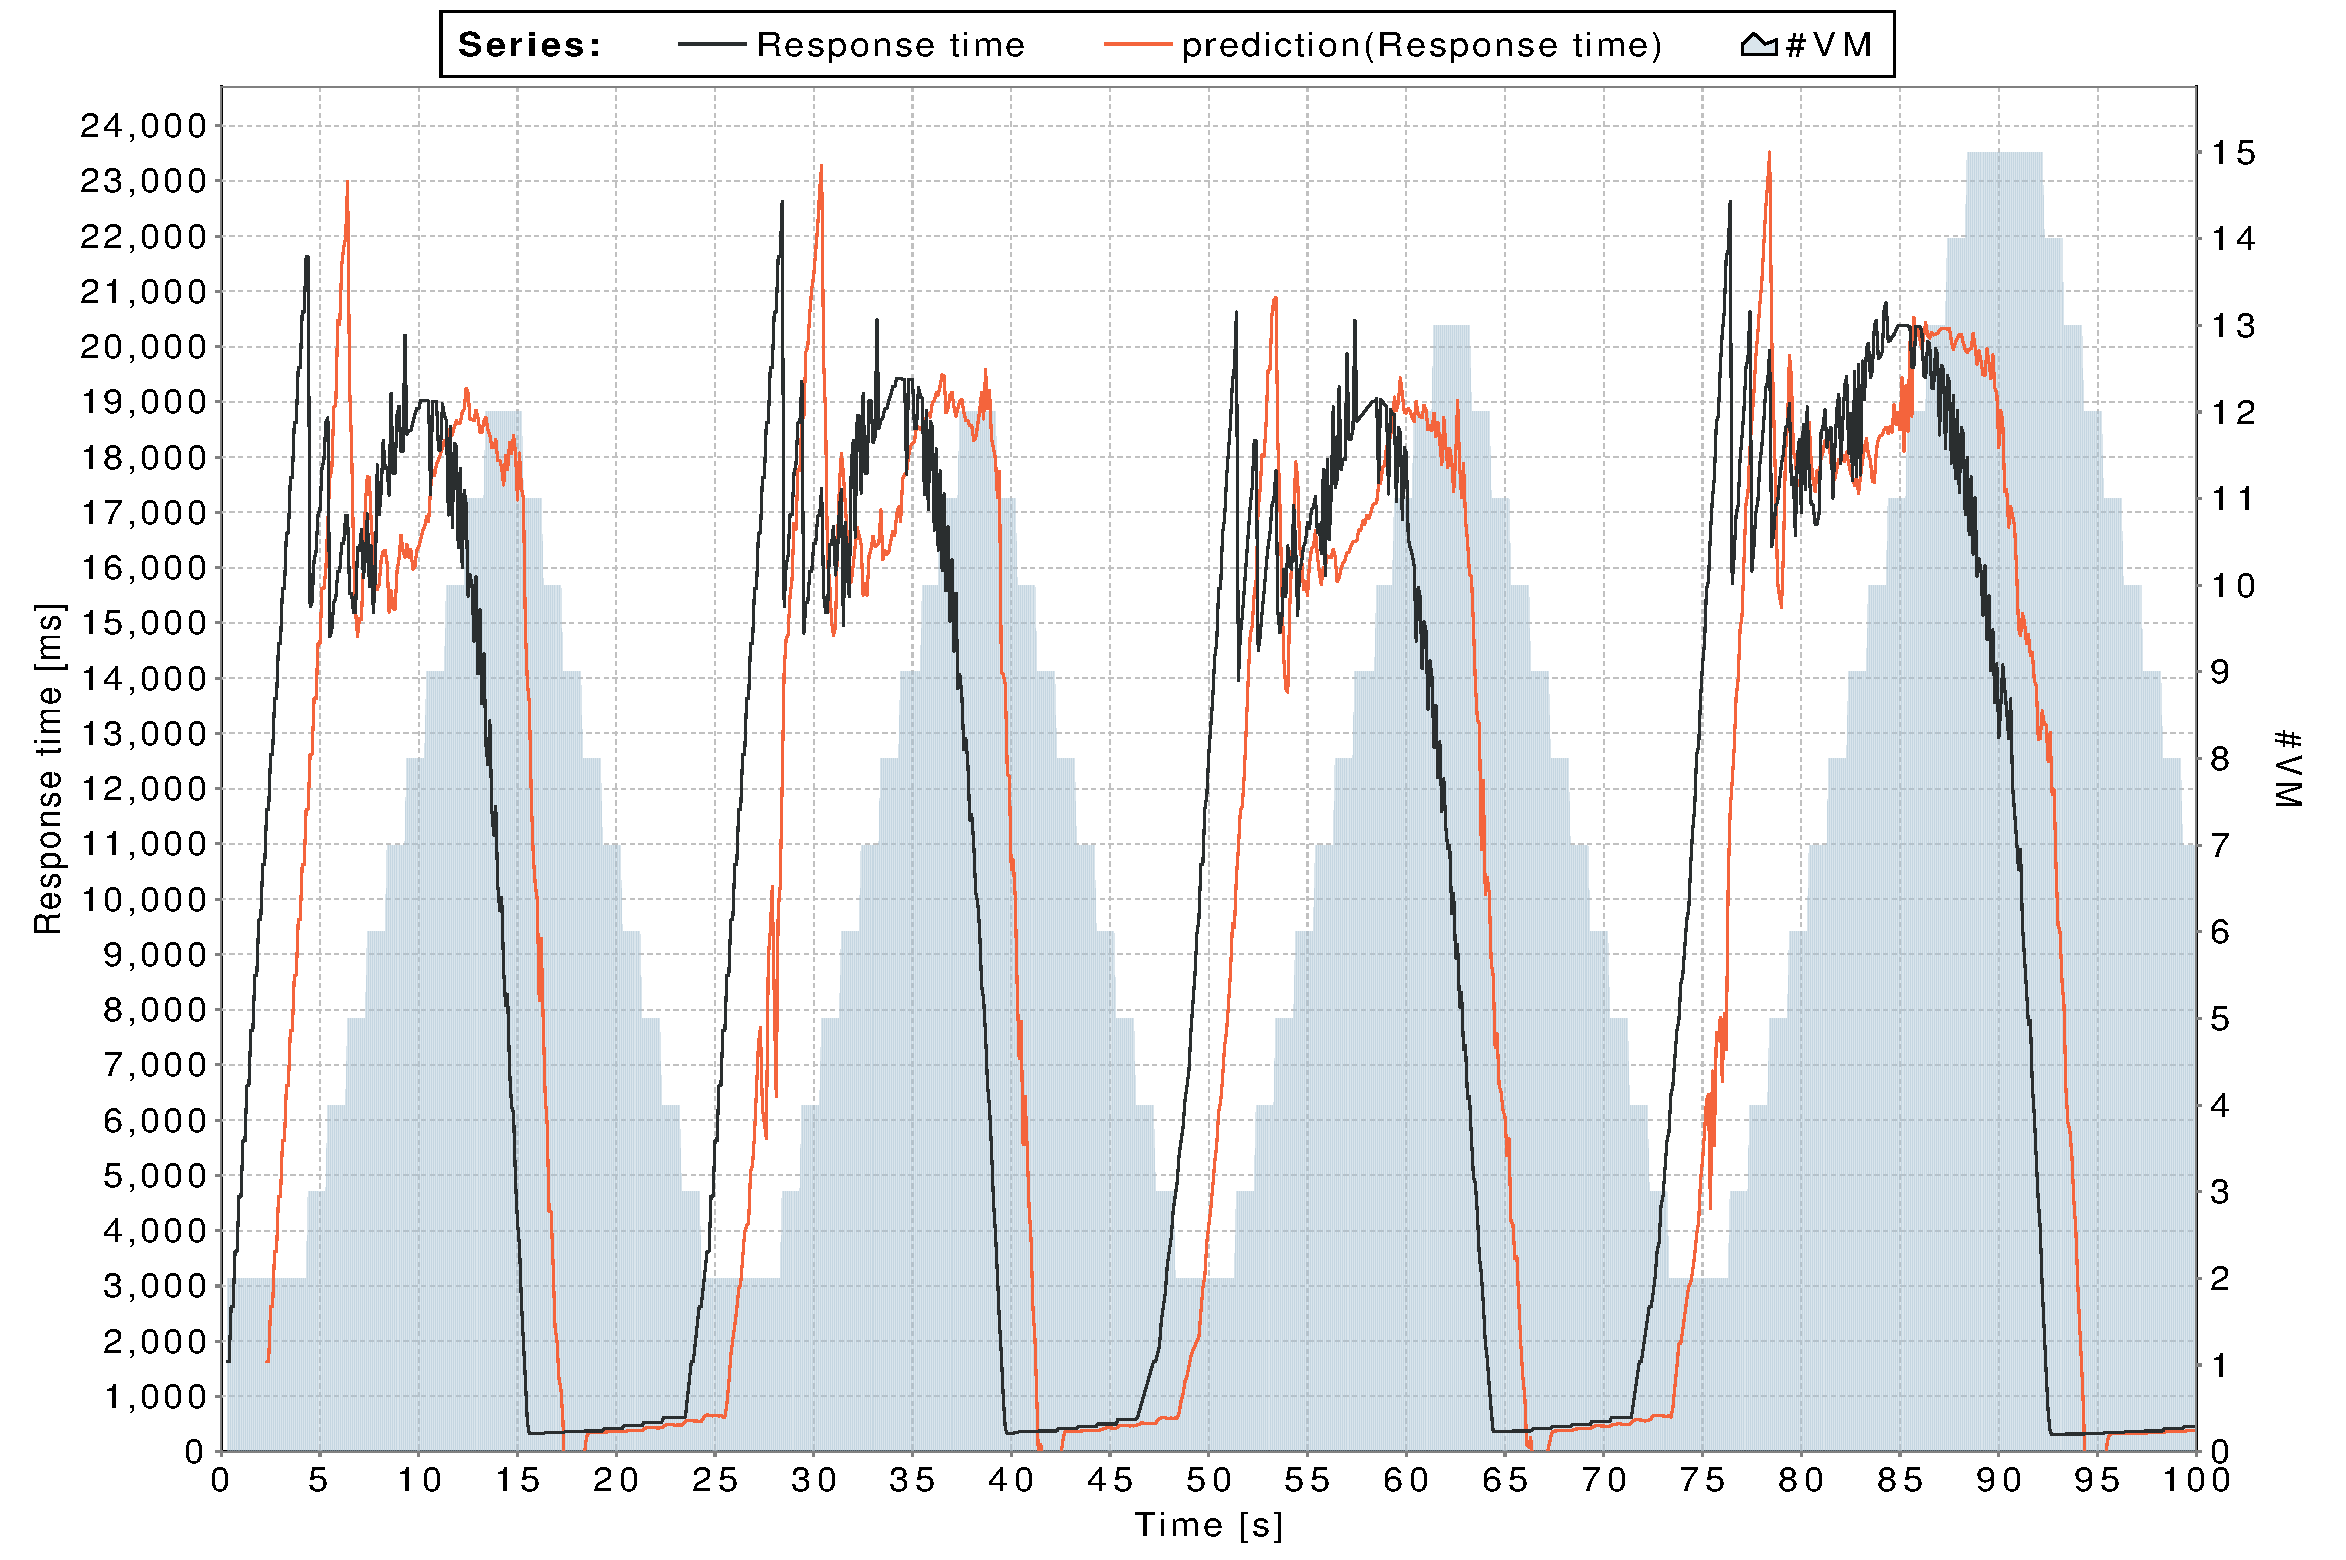
\includegraphics[width=0.40\textwidth]{chapters/chapter5/fig/NN1_1}
	\end{center}
	\caption{NN Scenario 1: 0s-100s}
	\label{fig:NN1_1}
\end{figure}

\begin{figure}[ht]
	\begin{center}
		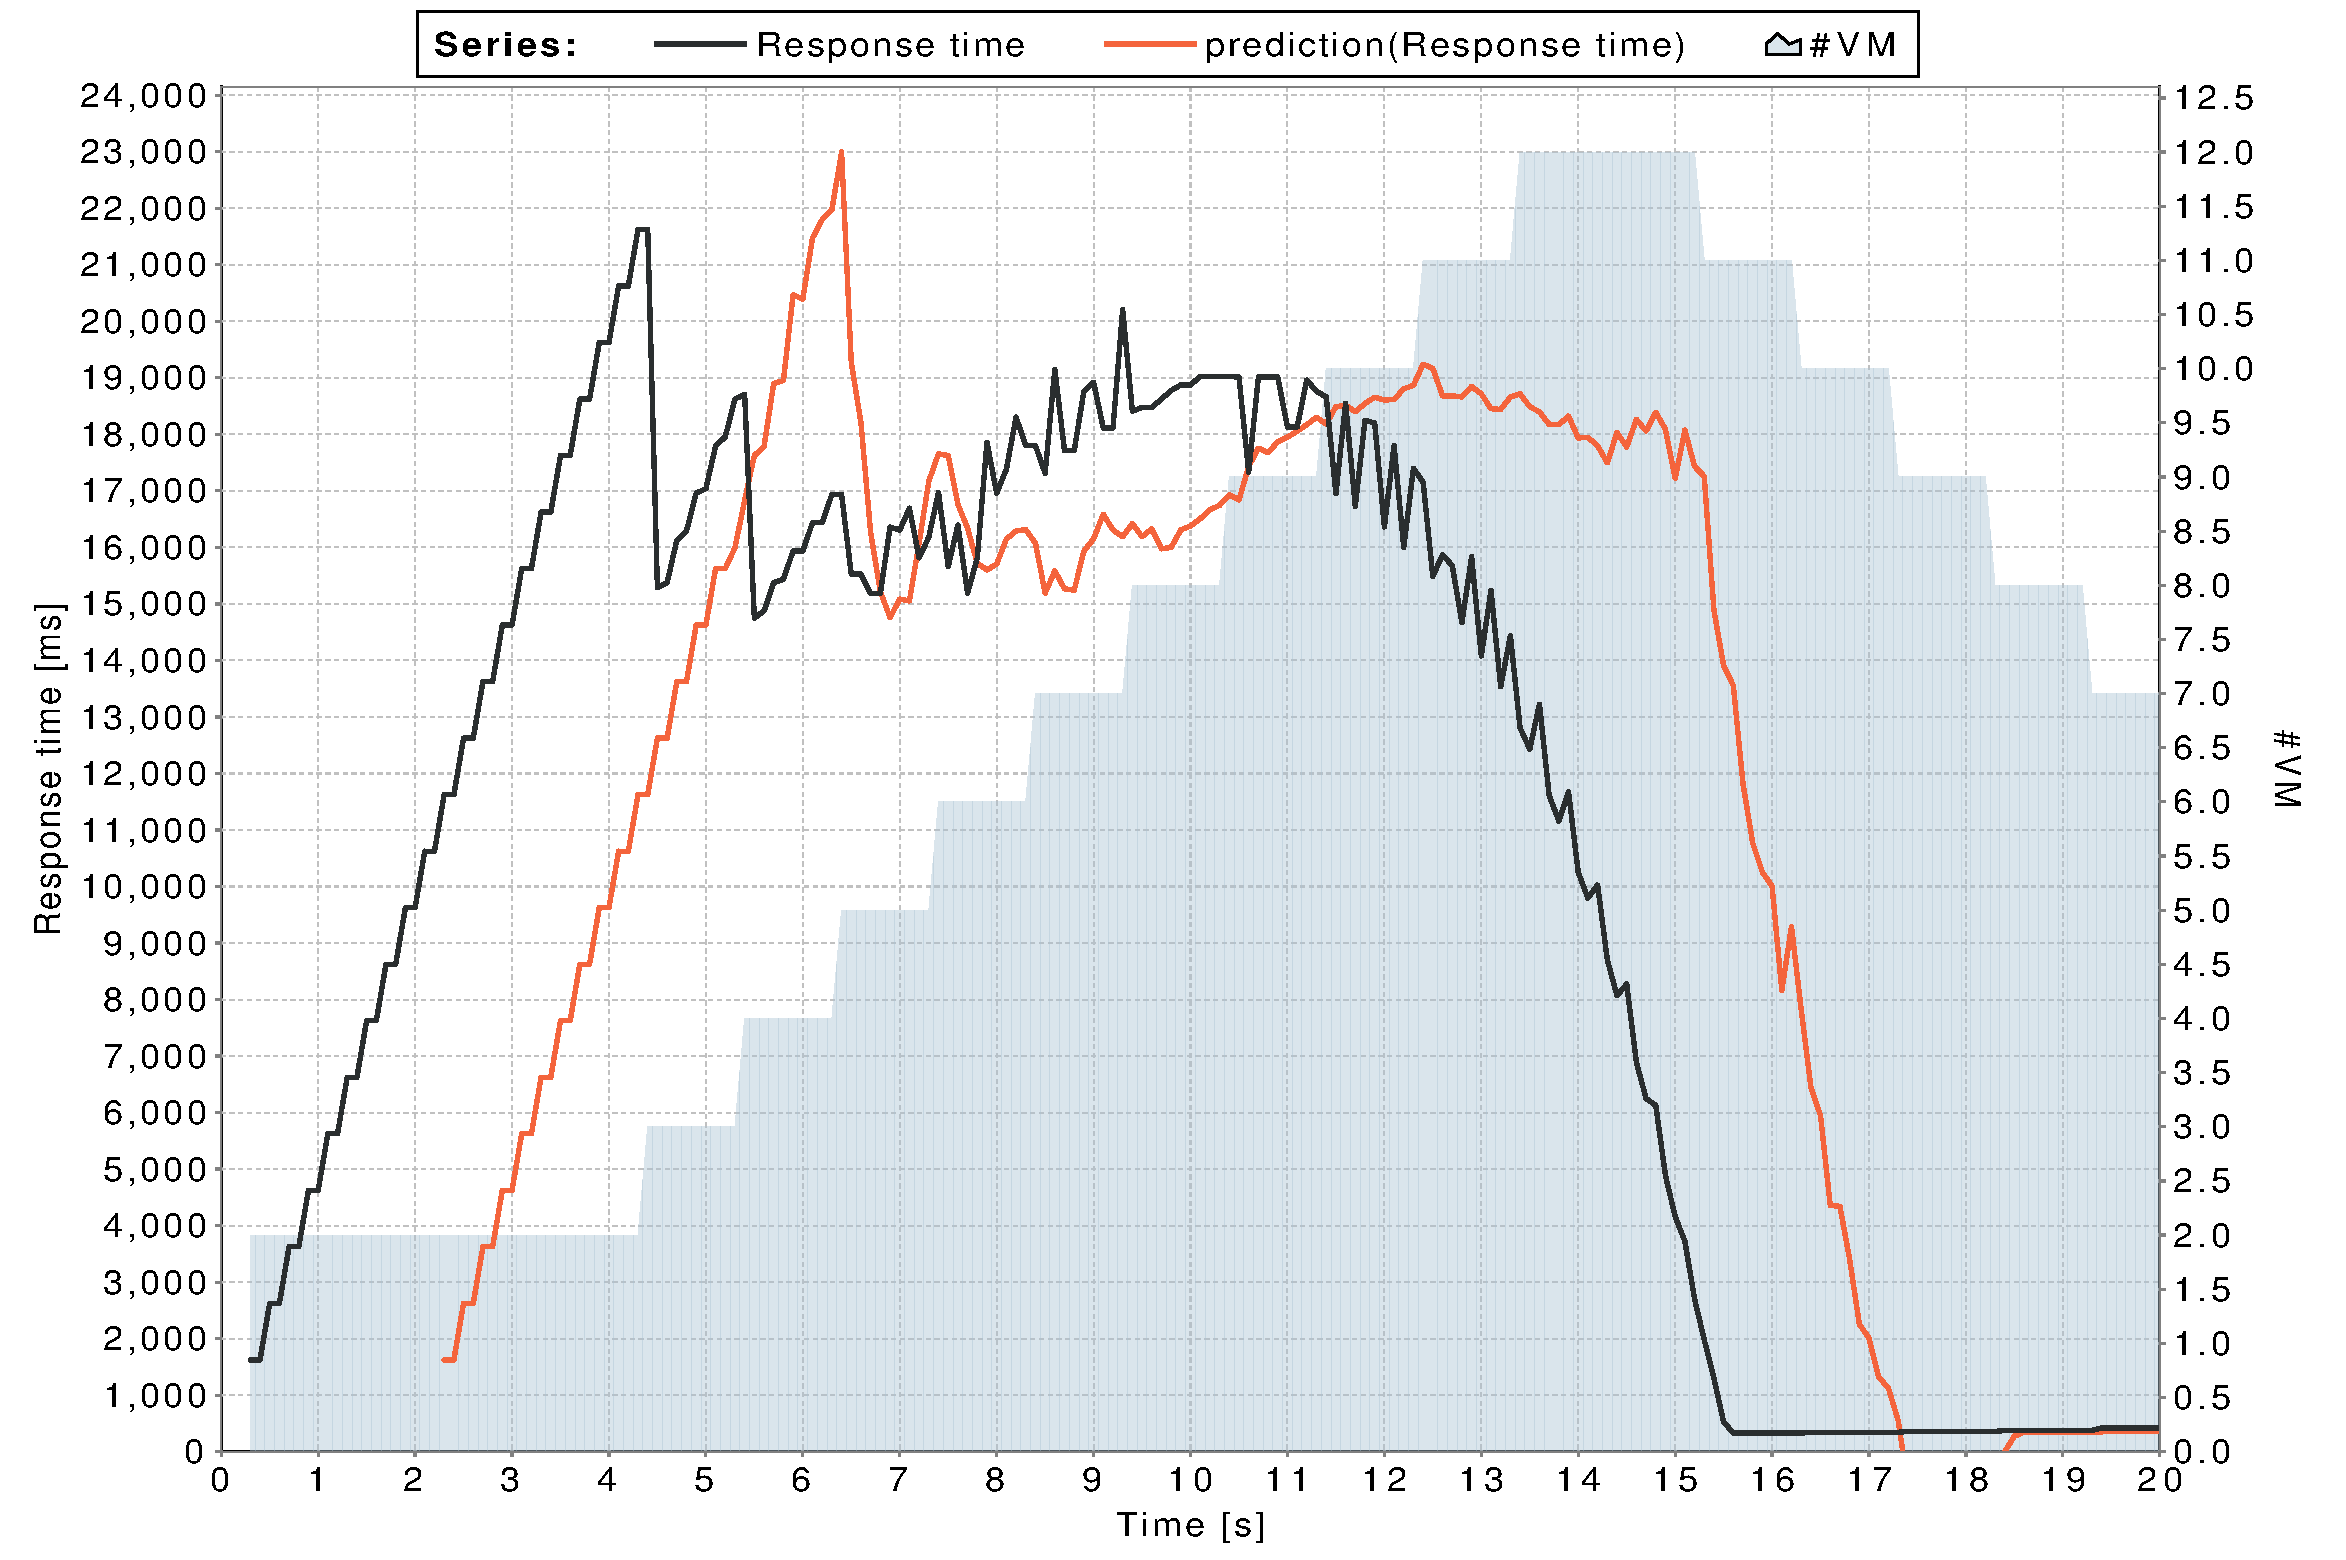
\includegraphics[width=0.40\textwidth]{chapters/chapter5/fig/NN1_2}
	\end{center}
	\caption{NN Scenario 1: 0s-20ss}
	\label{fig:NN1_2}
\end{figure}

\begin{itemize}
\item \textit{Neural Network:} In figure \ref*{fig:NN1_1} it can be seen, that the NN overestimates the peak of the burst loads in every case. Also it can be seen that the difference between predicted peak and real peak is the biggest during the first burst and that there is an improvement when predicting the later peaks of the bursts. The briefly following decline and rise after each peak, e.g., during sec 8-15 is respectively underestimated and overestimated but it can clearly be seen that there is an improvement in the last iteration. Figure \ref*{fig:NN1_2} shows the delay characteristics and that the algorithm in general can adapt well to the problem. 


\begin{figure}[ht]
	\begin{center}
		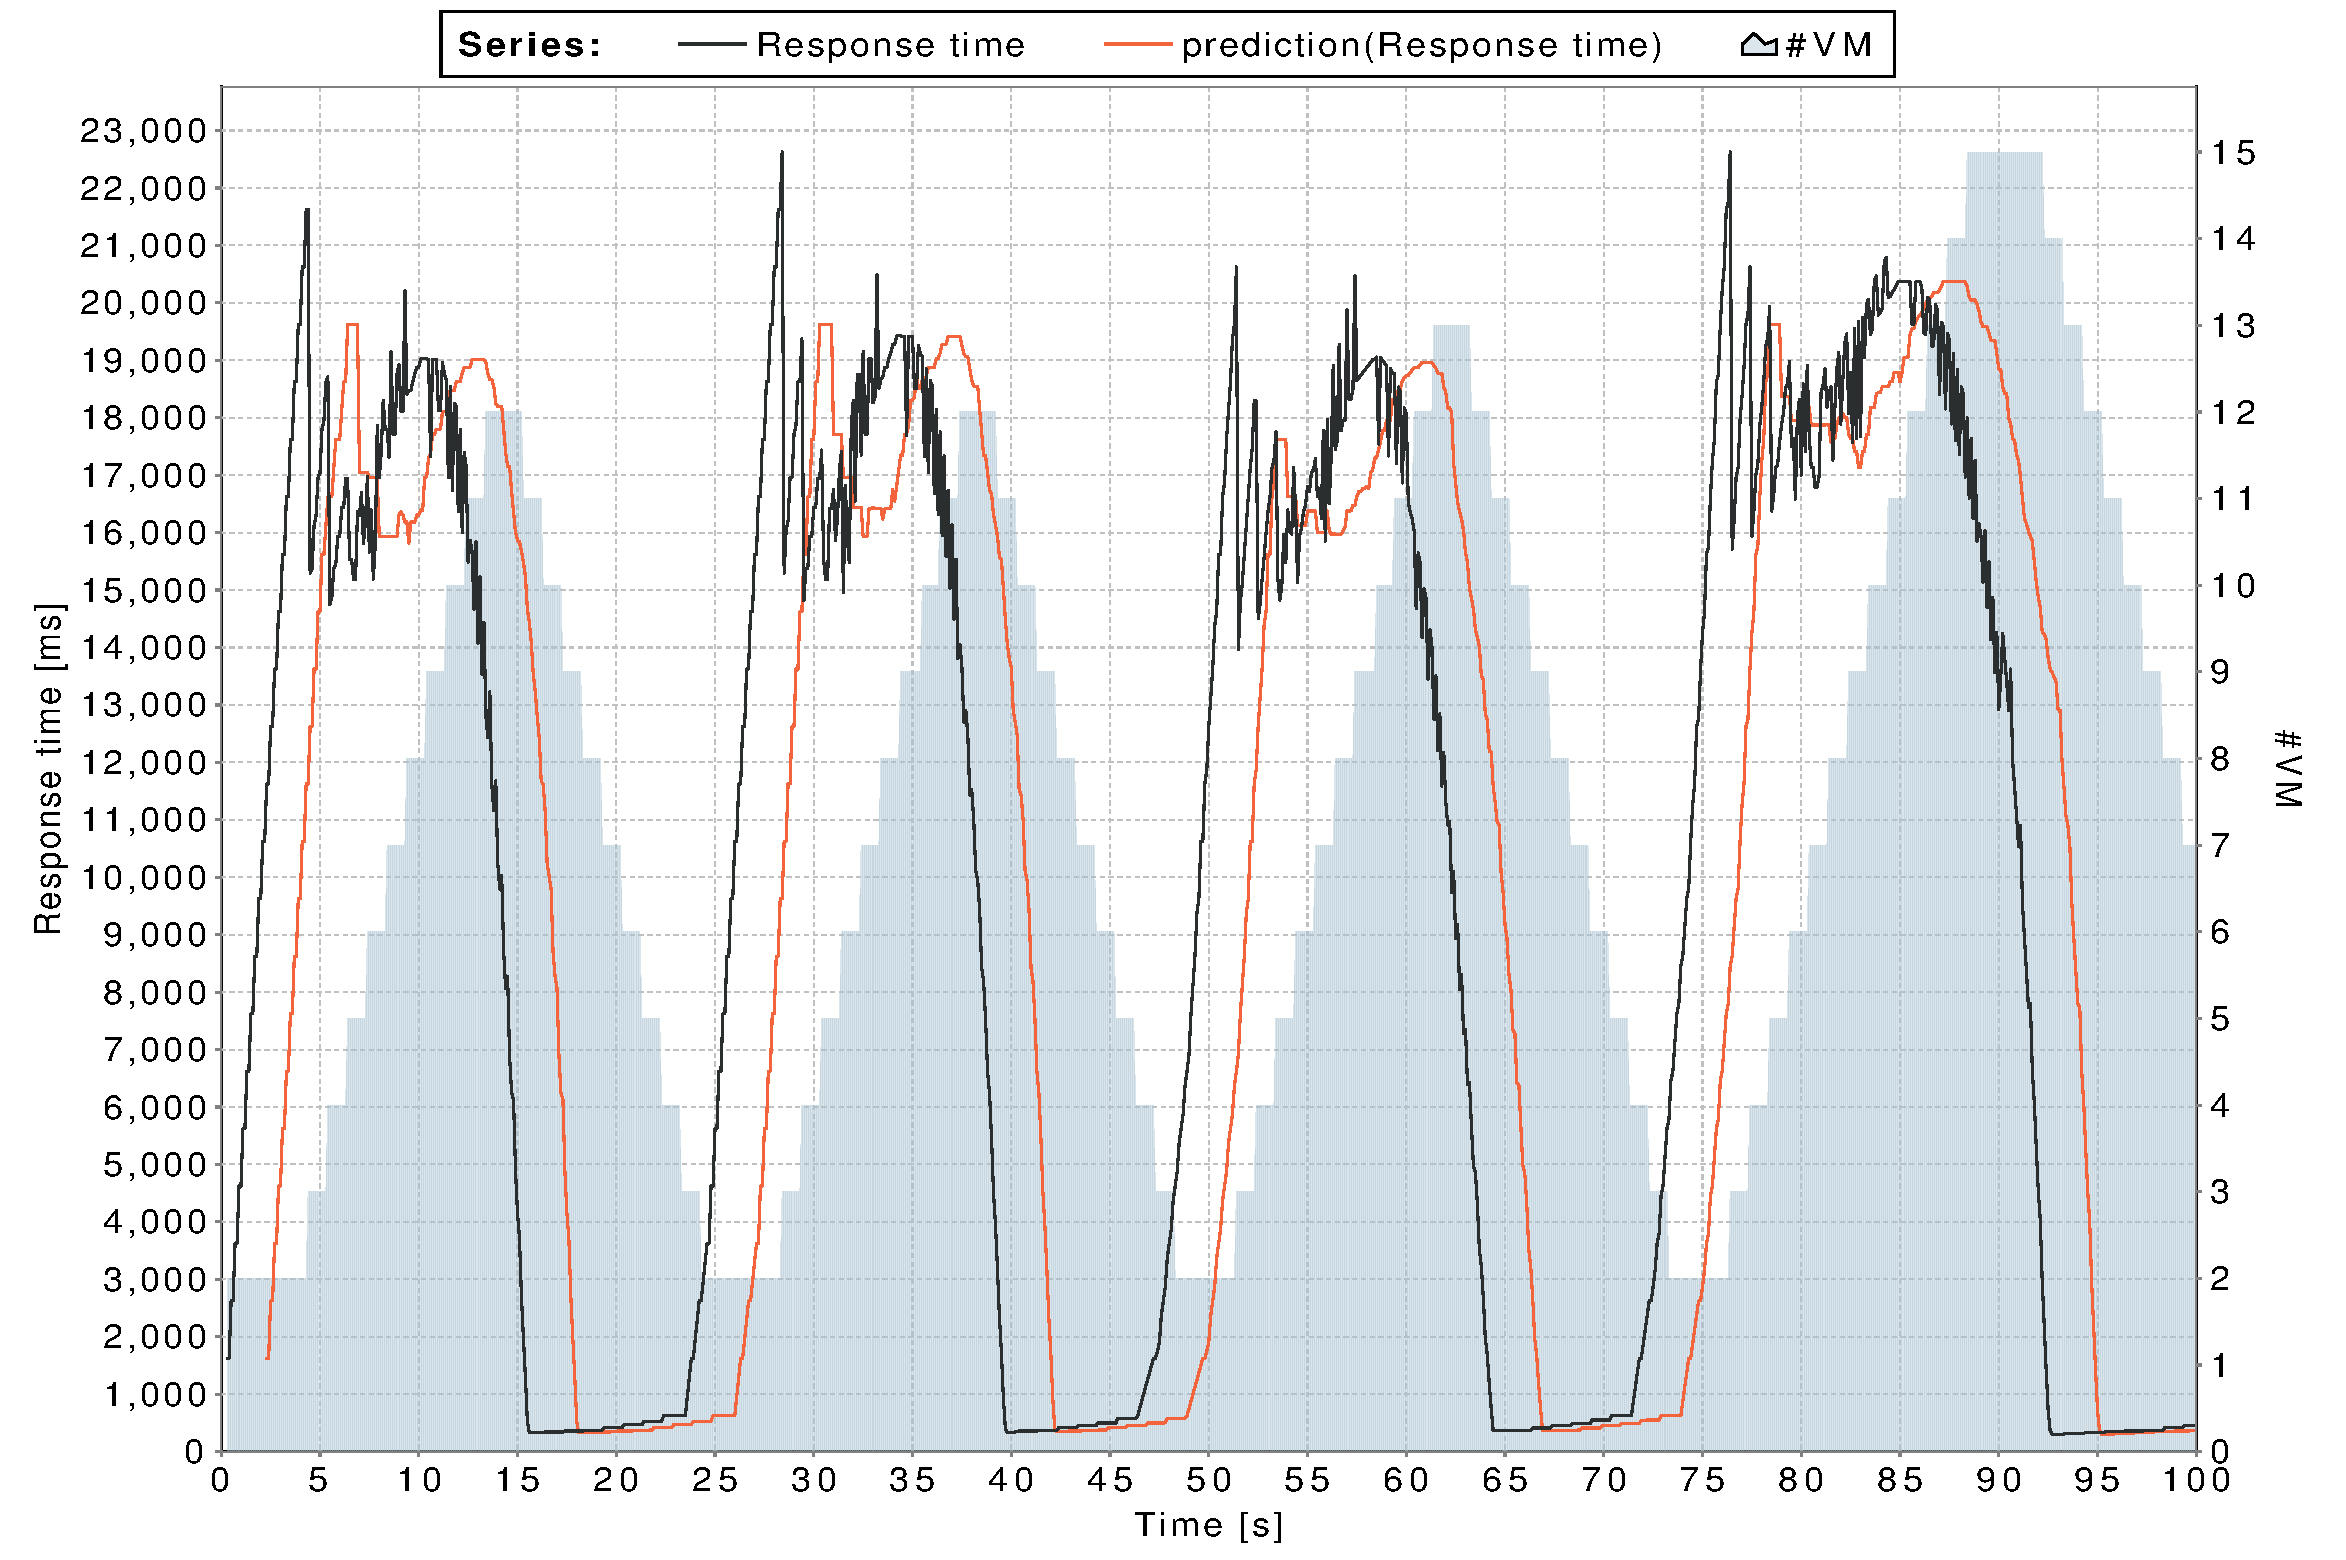
\includegraphics[width=0.40\textwidth]{chapters/chapter5/fig/SVM1_1}
	\end{center}
	\caption{SVM Scenario 1: 0s-100s}
	\label{fig:SVM1_1}
\end{figure}

\begin{figure}[ht]
	\begin{center}
		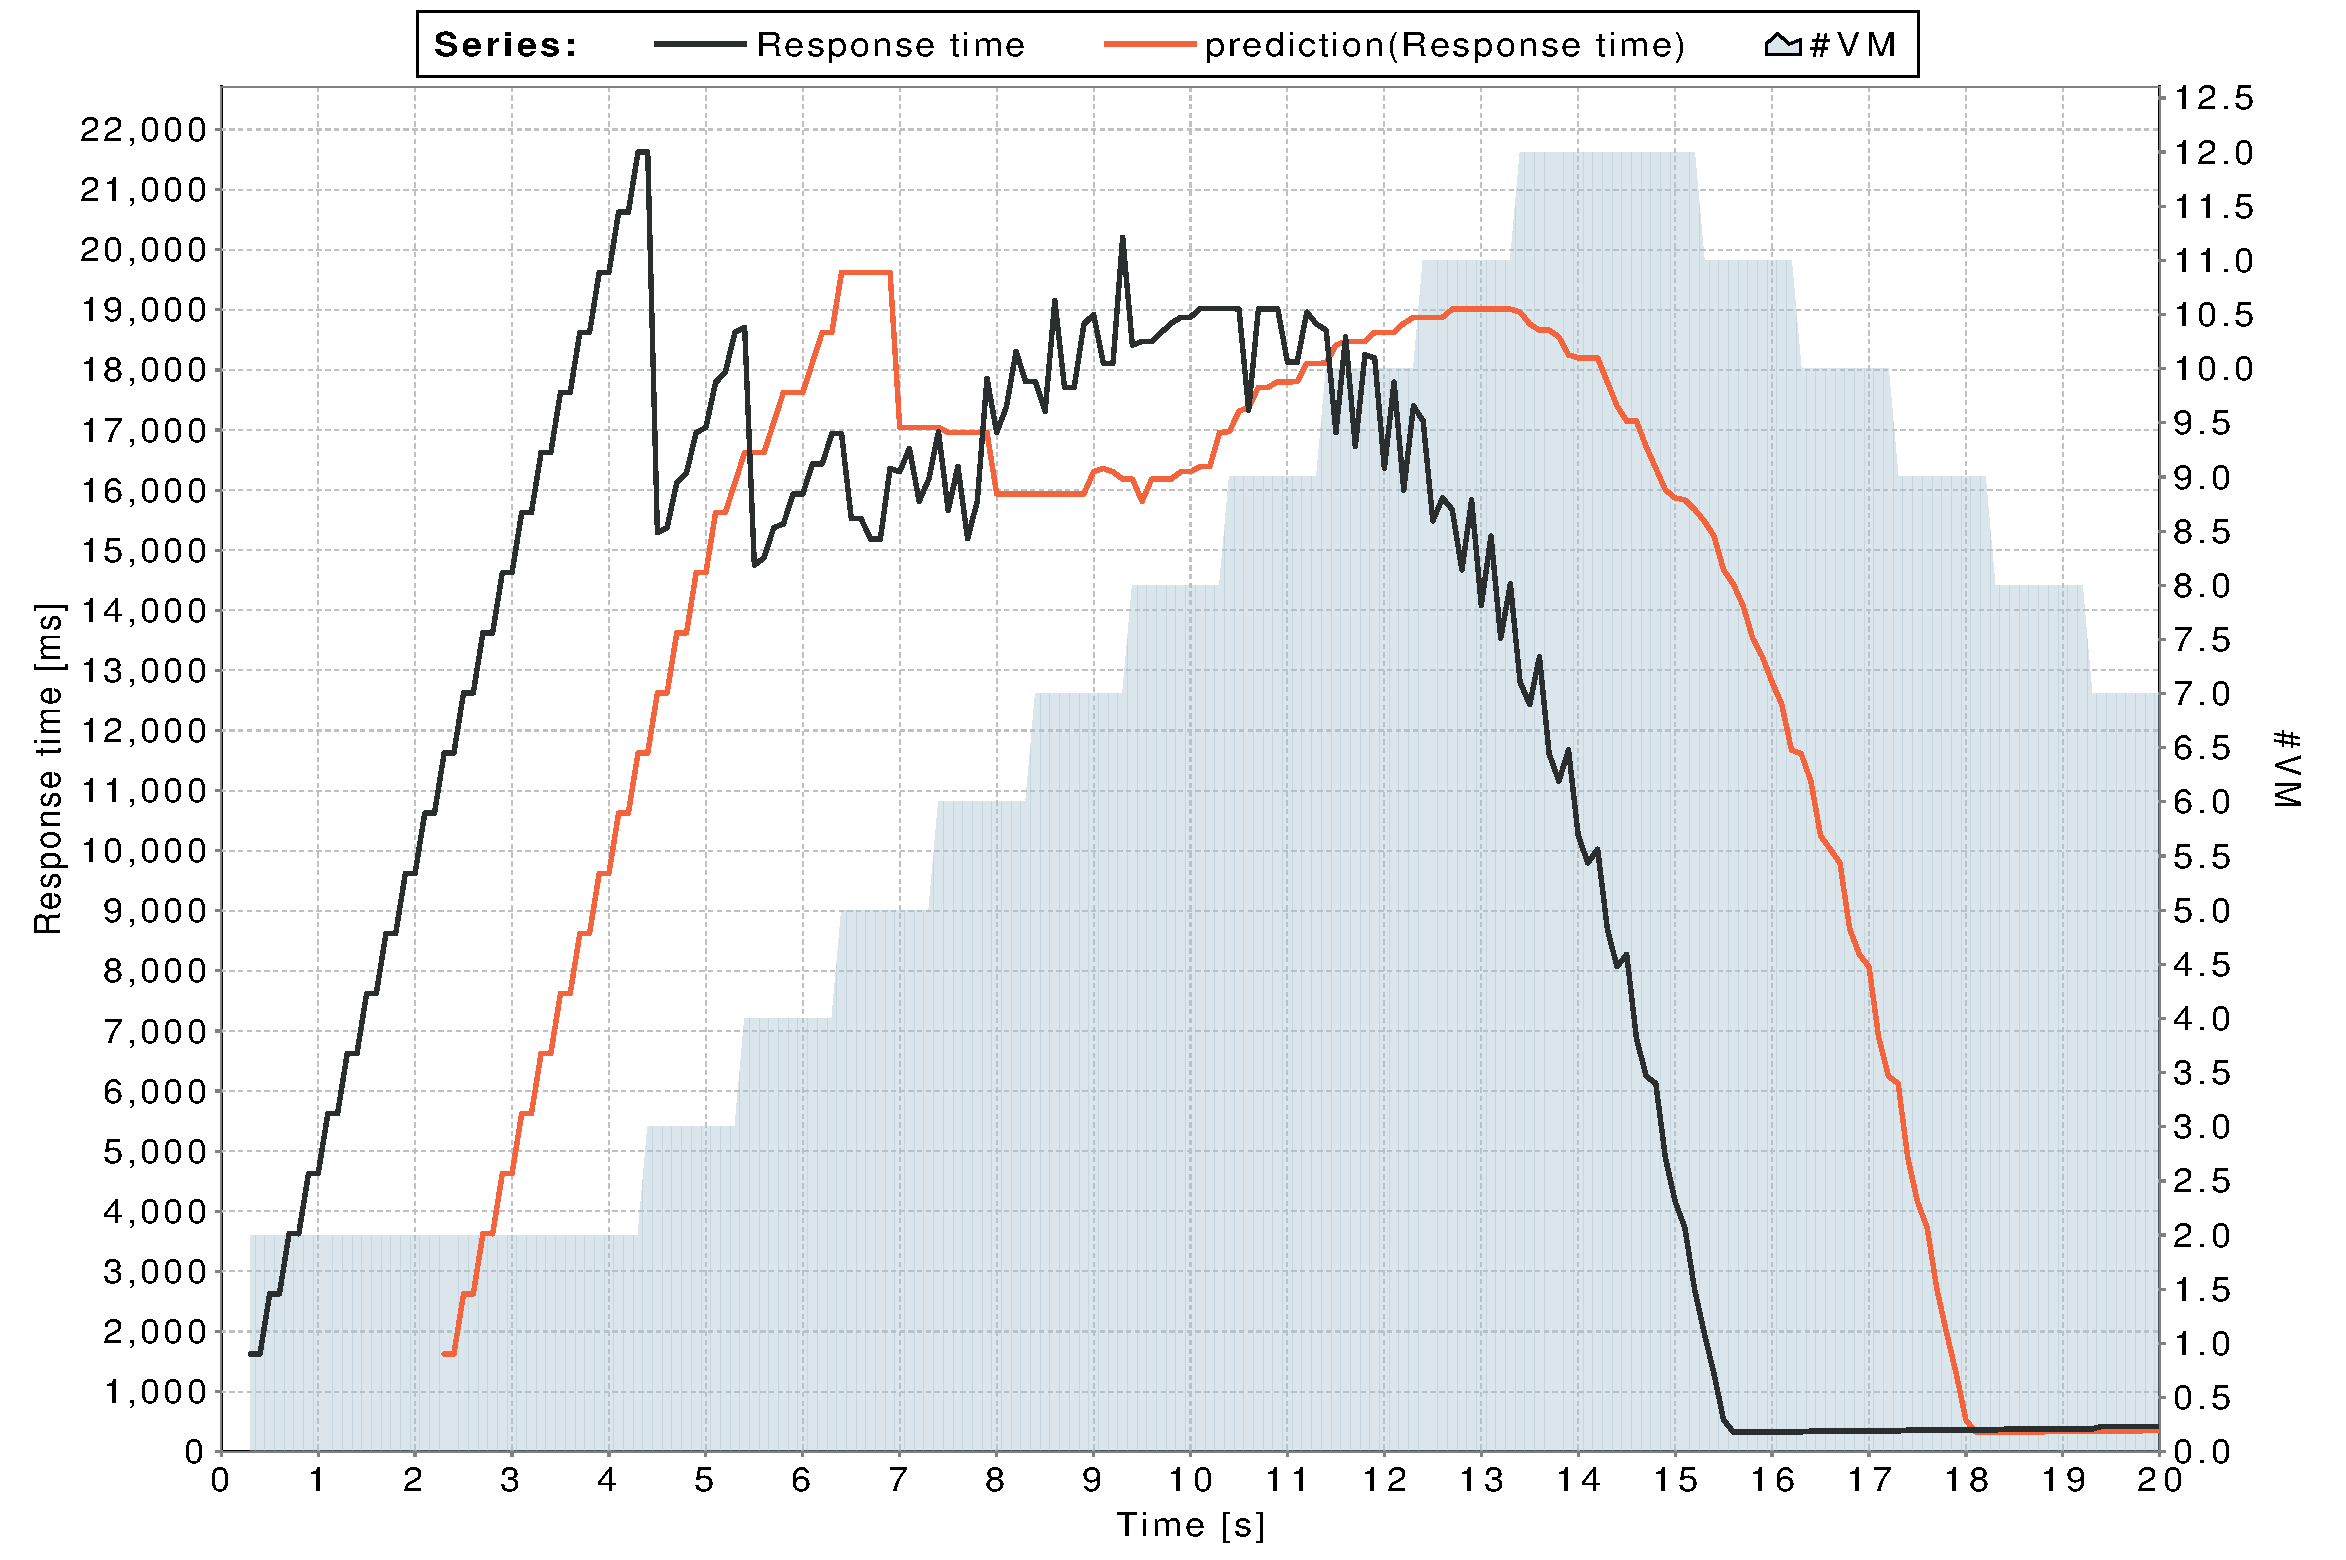
\includegraphics[width=0.40\textwidth]{chapters/chapter5/fig/SVM1_2}
	\end{center}
	\caption{SVM Scenario 1: 0s-20ss}
	\label{fig:SVM1_2}
\end{figure}

\item \textit{Support Vector Machines:} Figure \ref*{fig:SVM1_1} shows a contrast to the NN algorithm. In the case of SVMs the first peak of each burst is underestimated. The following cooldown phase before the second peak of each burst is overestimated but an improvement over time can be seen, especially on the last burst. Figure \ref{fig:SVM1_2} looks specifically at the first burst and a comparison to the NN \ref*{fig:NN1_2} makes it clear that SVMs predict a more smooth curve. It should be kept in mind that it is realistic to assume that in real life there are scenarios with different requirements regarding the reaction to those predictions where this specific differences, smooth or rough, could be seen as either an advantage or disadvantage.


\begin{figure}[ht]
	\begin{center}
		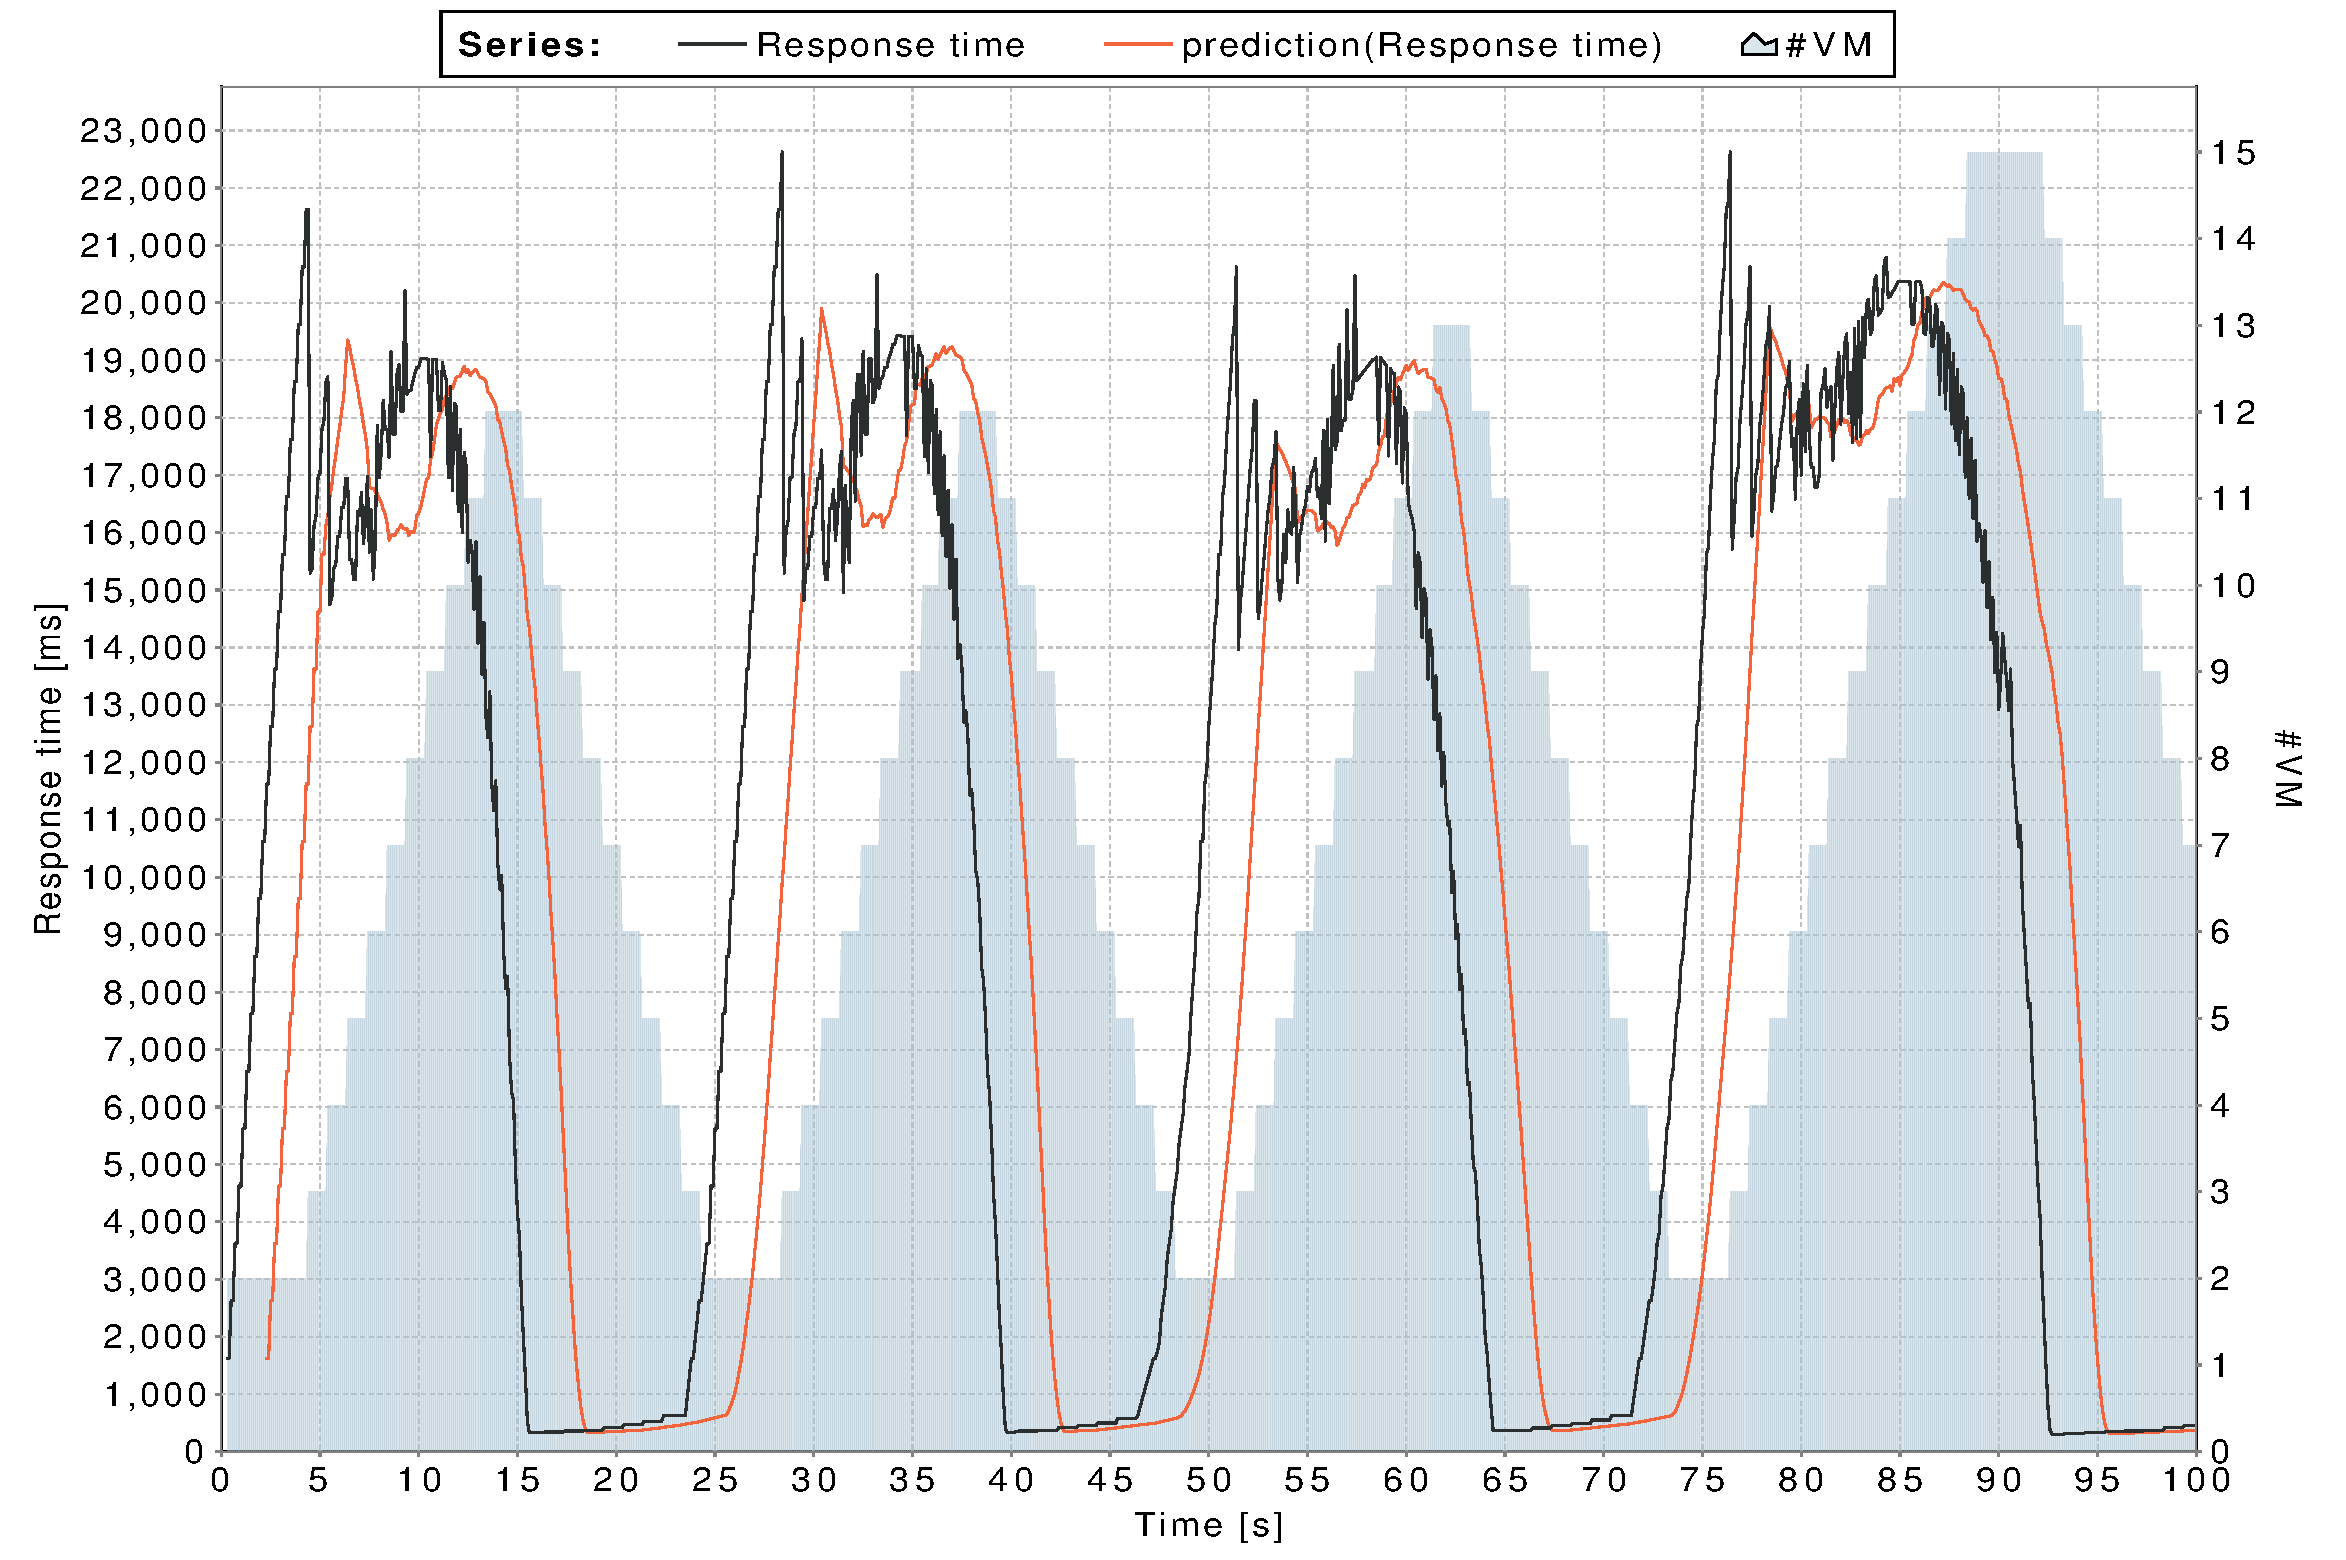
\includegraphics[width=0.40\textwidth]{chapters/chapter5/fig/LR1_1}
	\end{center}
	\caption{SVM Scenario 1: 0s-100s}
	\label{fig:LR1_1}
\end{figure}

\begin{figure}[ht]
	\begin{center}
		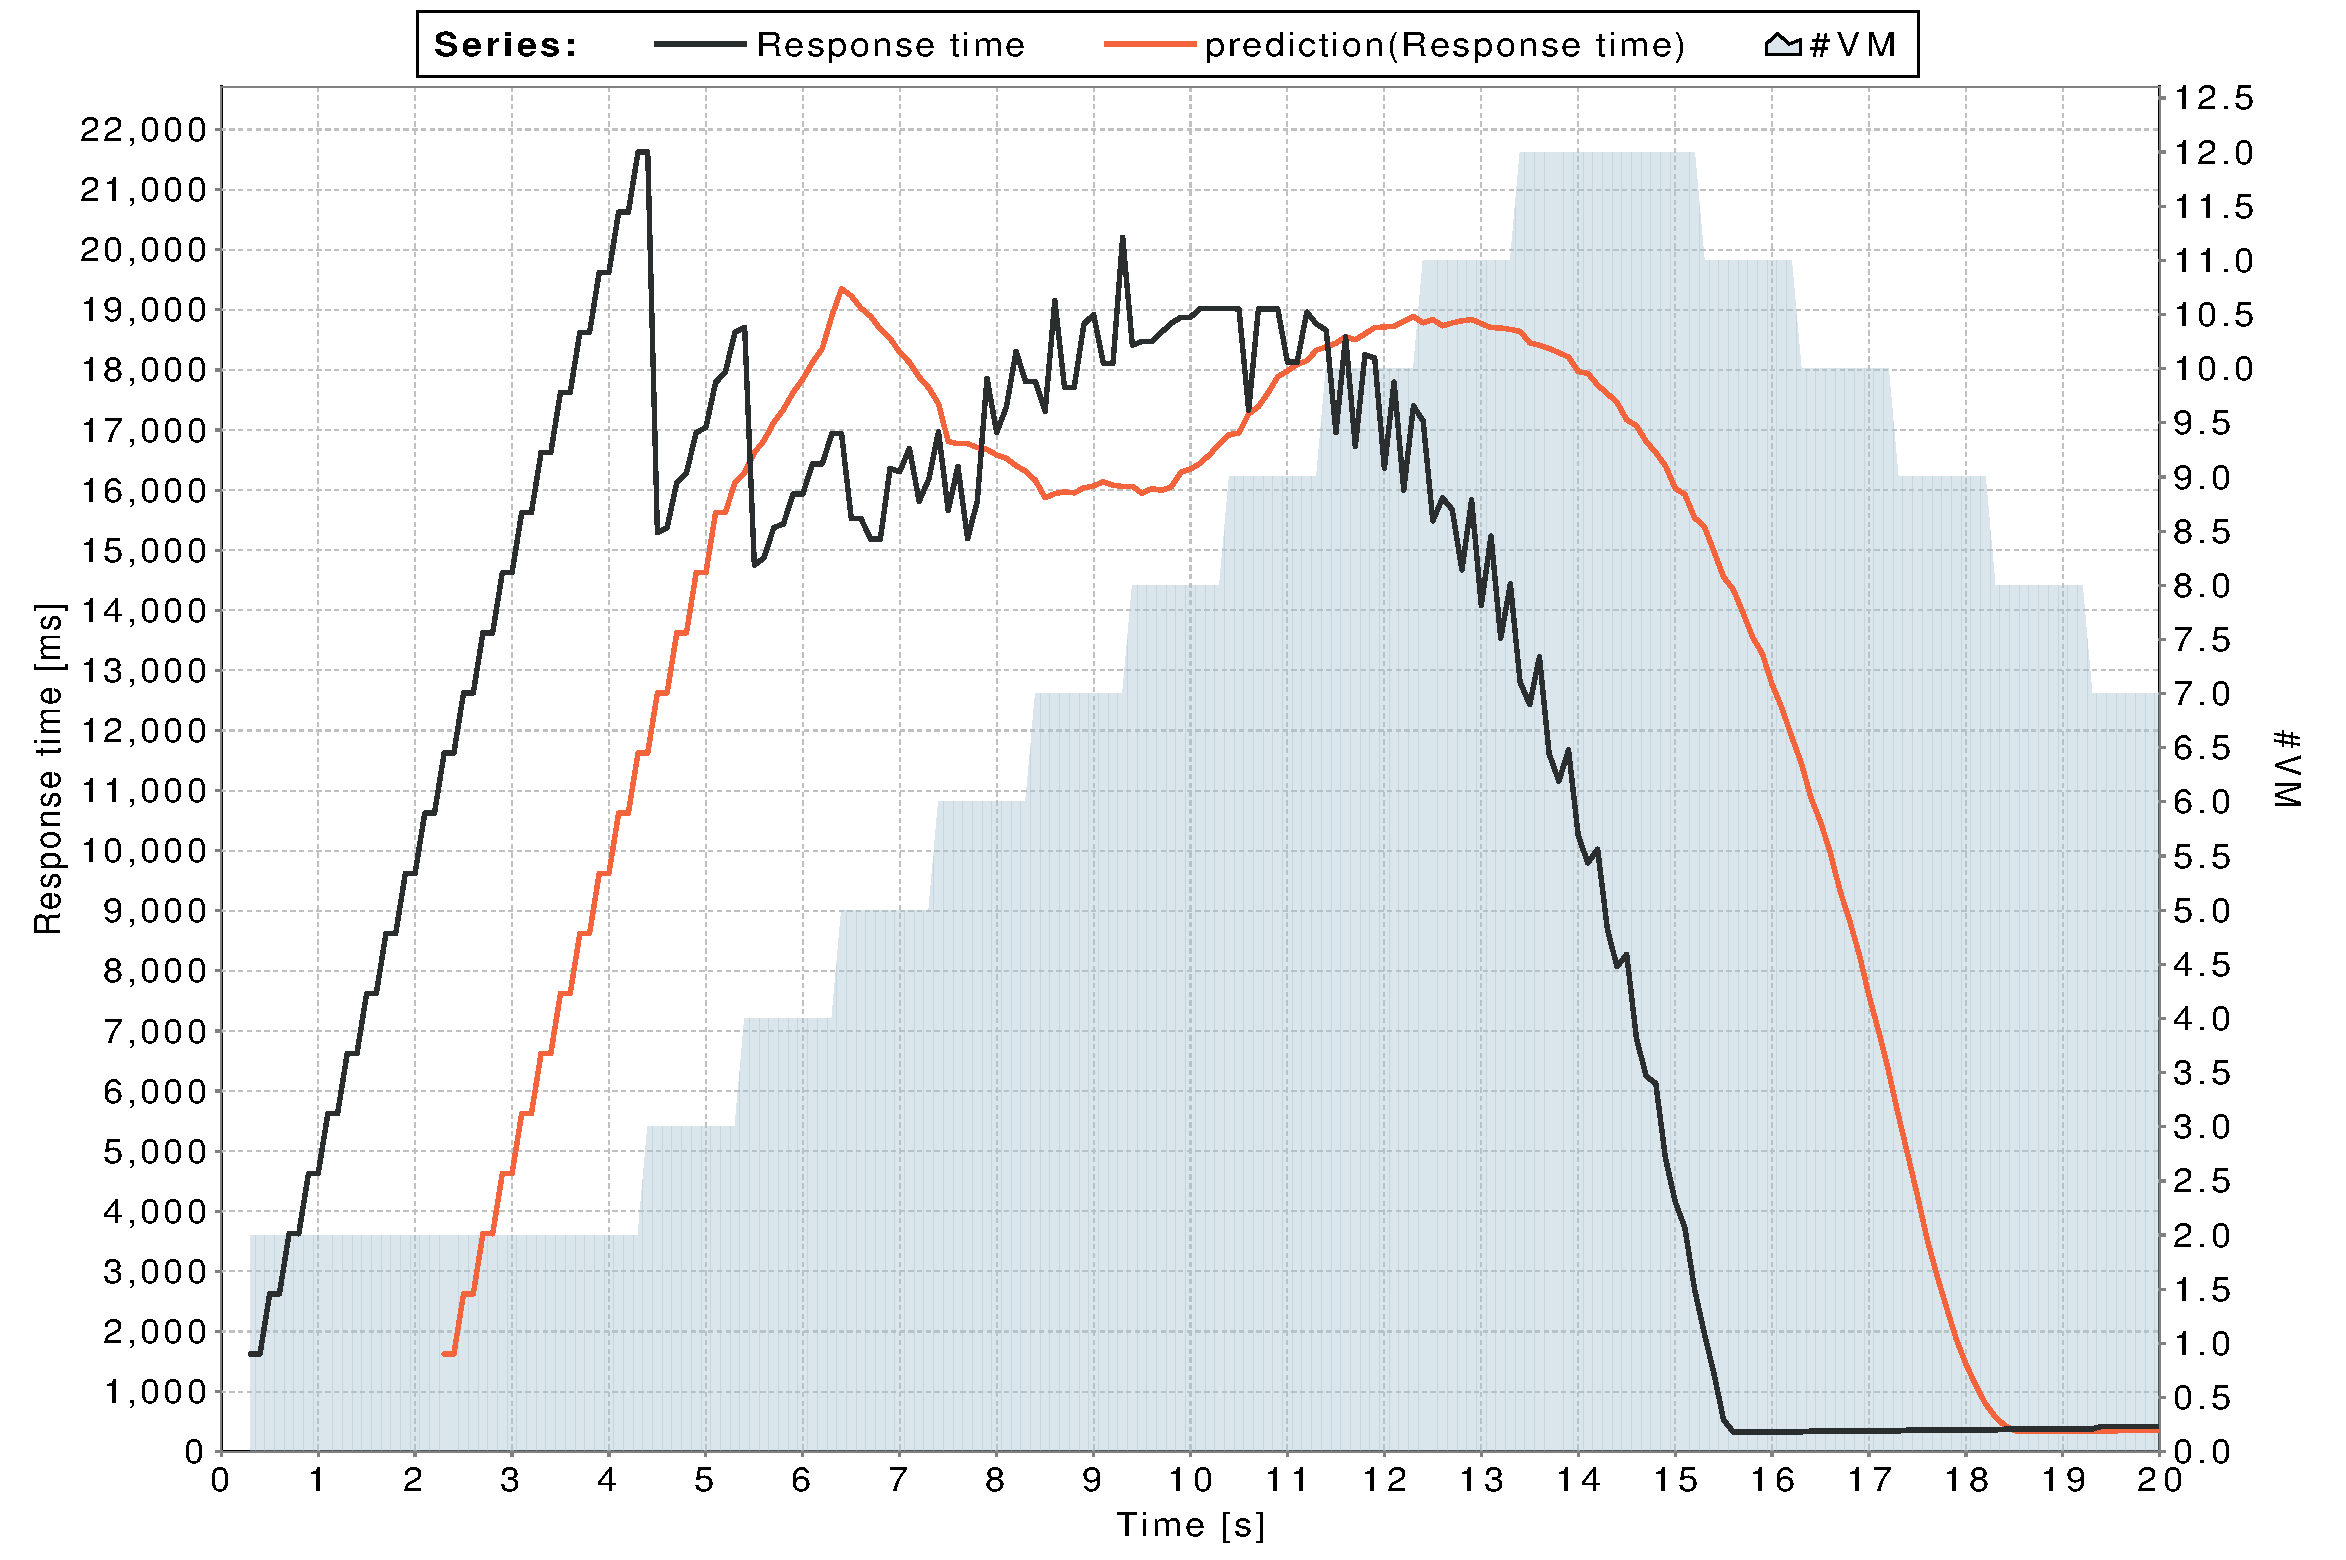
\includegraphics[width=0.40\textwidth]{chapters/chapter5/fig/LR1_2}
	\end{center}
	\caption{SVM Scenario 1: 0s-20ss}
	\label{fig:LR1_2}
\end{figure}

\item \textit{Linear Regression:} The predictions made with the help of a Linear Regression learner shown in figure \ref*{fig:LR1_1} seem to be very similar to those predictions made by the SVM in figure \ref*{fig:SVM1_1}. This insight is further substantiated by taking a closer look at the bursts in figure \ref*{fig:LR1_2} and figure \ref*{fig:SVM1_2} where a similar prediction pattern can be seen. Worth mentioning is that the predictions made by Linear Regression lead to an even smoother curve compared to the curve predicted by the other 2 algorithms.
\end{itemize}

\paragraph*{Scenario 2}
The second scenario shows a system with a normal usage load. The load slowly builds up and then slowly decays again. This scenario in this form or alternatively with strongly decaying load at the is a normal use of the system such as a file transfer or the curl of an larger API.  The scenario duration of twenty seconds is in the normal real life range for such actions. This load is easier to scale because the duration and therefore the speed needed to process this is lower.

\begin{itemize}
\item \textit{Neural Network:} When looking at the overview in Figure 7 it is demonstrated that moderate changes in response times are learned rather well. The interesting part, shown in more detail in Figure 8, showcases the nature of overestimation. Again, the peak is overestimated, but the predicted curve recovers very fast and yet this issue occurs again after the second plateau. It should be noted that with a different configuration of the NN algorithm a very different curve can be predicted. For this paper we looked at a specific configuration of the algorithm because this characteristic can be utilized and will be explained during the comparison of the algorithms.

\item \textit{Support Vector Machines:} The overview shown in Figure9 displays the capability of the algorithm to be able toa dapt to a singular, steadily climbing response time. The prediction during the first phase (0-60s) is handled well by the algorithm. Figure 10 illustrates that the spontaneous and large decline in response time is learned very well. This is an important characteristic as predictions based on those quick changes couldbethefocusduringtheapplicationinreal-timescenarios. None of the other algorithms is able to predict scenario 2 this precisely.

\item \textit{Linear Regression:} Figure 11 shows again great similarity between predictions made with the help of Linear Regression and SVMs. Again the difference is that the ascent of the curve is predicted in a smoother way. Additionally, the spontaneous and large decline seen in Figure 12 is not predicted very well. The same characteristic applies on the following smaller decline. As a conclusion it can be said that in this specific scenario the model trained by LinearRegression is the weakest. 
\end{itemize}

\textbf{Scenario 3} 
The third and final scenario is a mixture of the two previous ones. First, a single burst is triggered, followed by a slower but higher load, which decreases in the end. Such mixed load profiles are very often found in reality because different users and systems access resources at the same time. These loads are not synchronized and therefore can lead to chaotic scenarios.

\begin{itemize}
\item \textit{Neural Network:} Figure 13 shows that during the first phase (0-100s) the model trained by a NN has minor problems in predicting the response time. Although the peaks are generally predicted well, sometimes they are underestimated and sometimes overestimated. But in contrast to the other algorithms the difference in error margin is very small in most cases. During the recovery times after each slope, the local minima are overestimated almost in every case. While the first big peak of a response time over 42000ms is overestimated as well, the second one is predicted almost perfectly. The relative smooth slopes before, during and after the larger peaks are predicted very well with no prominent deficit. 

\item \textit{Support Vector Machines:} Figure 14 shows that a model trained by SVMs can predict the response time for a varying scenario rather well. The occurring peaks during the first phase (0-100s) are underestimated in every case, but not to a large degree. This leads likewise to the underestimation of the recovery times after each peak, which are the consequence of adding and deleting Virtual Machines. The two larger peaks with a response time of over 42000ms are underestimated again by a small margin while the relative smooth slopes before, inbetween and after are learned well with noprominent deficit in their prediction. 

\item \textit{Linear Regression:} Figure15 shows that a model trained by Linear Regression can cope well in a varying scenario. Similar to the SVM model it slightly underestimates the response time in the first phase (0-100s). In general, it can be said that those models are very similar and have only minor, negligible differences. The main difference is that the use of Linear Regression leads to smoother slopes.
\end{itemize}

While it was shown that all 3 algorithms can be effectively used for predicting the response time in different scenarios it can be said that the NN has a minor advantage over the other algorithms. The main reason is that the NN, in general, slightly overestimates and almost never underestimates the response time. The practical application of this knowledge, e.g., using those predictions in combination with a scaler who manages the quantity of VMs leads to a more assuring state that requirements like defined SLAs can be covered more carefully than with other algorithms. In less critical businesscases, where the defined SLAs and response times are not that sensitive, the other 2 algorithms, SVMs and Linear Regression, can be used despite their tendency to slightly underestimate response times. Especially the Linear Regression with its fast training and deployment times could be considered in near real-time scenarios.


%\section{Simulator}
%\subsection*{Requestgenerator \& Load Balancing}
%\subsection*{Cloud SIM}
%\subsection*{Log \& Reporting}

\section{Holistic SLA Management}
As  described in the previous sections, the quality, respectivly the KPIs of a service can be improved by the described methods. However, it is not enough to concentrate merley on the quality of the individual services, since in modern cloud landscapes, disruptions, failures or performance issues can occur. This requires a holistic approach, where the management of the individual service quality and the overall management of the cloud in brought together. For example, in a general cloud landscape it is quite possible that the individual services are scaled and managed almost optimally by the algorithms described above, but the overall performance of the landscape is the limitating factor. This is where the holistic SLA management comes to bear. Here, not only on each service as a single is respected but also the overall situation of the landscape is taken care of. For example, in an cloud enviornment where the performance is adversely affected by an infrastructure problem, this may mean that certain services are sacrificed in favor of other services. In particular, the contractual penalties and categorization of the customer regulated by the SLAs play an overriding role.


\subsection{Instance Sheduling with Genetic Algorithm}

\section{Results and Evaluation}

\subsection{Scenario A}
Request Response time SLA


\subsection{Scenario B}
HDD and Backup SLA

\subsection{Scenario C}
SLA Management to Cost / Fine minimization